\documentclass[a4paper,12pt,twoside]{report}
%%%%%%%%%%%%%%%%%
%% PACKAGES
%%%%%%%%%%%%%%%%%
\usepackage[utf8]{inputenc}
\usepackage[T1]{fontenc}
\usepackage[french]{babel}
\usepackage{xcolor}
\usepackage{hyperref}
\hypersetup{colorlinks,
	citecolor={red},
	urlcolor={blue},
	linkcolor={blue},
	breaklinks={true},
	pagebackref={true},
	hyperindex={true},
	pdfauthor={BOSOLINDO EDHIENGENE Roger}
}
\usepackage{url}
\usepackage{enumitem}
\usepackage{multicol}
\usepackage{tocbibind}
\usepackage[printonlyused]{acronym}
\usepackage{cite}

\usepackage{xcolor}
\usepackage{listings}

\lstdefinestyle{python}{
    language=Python,
    basicstyle=\ttfamily\small,
    keywordstyle=\color{blue}\bfseries,
    commentstyle=\color{gray}\itshape,
    stringstyle=\color{teal},
    numbers=left,
    numberstyle=\tiny\color{gray},
    frame=single,
    breaklines=true,
    showstringspaces=false,
    tabsize=4
}
\lstset{style=python}

\lstdefinestyle{arduino}{
	language=C++,
	basicstyle=\ttfamily\small,
	keywordstyle=\color{blue}\bfseries,
	commentstyle=\color{gray}\itshape,
	stringstyle=\color{teal},
	numbers=left,
	numberstyle=\tiny\color{gray},
	frame=single,
	breaklines=true,
	tabsize=4,
	morekeywords=[1]{setup, loop, pinMode, digitalWrite, analogWrite, analogRead, delay, begin, println, print},
	morekeywords=[2]{int, void, float, const, String, HIGH, LOW, OUTPUT, INPUT},
	keywordstyle=[1]\color{brown}\bfseries,
	keywordstyle=[2]\color{purple}\bfseries
}

%%	Maths
\usepackage{amsfonts,amsmath,amssymb,amsthm,mathrsfs}

\theoremstyle{definition}
\newtheorem{defi}{Définition}
\newtheorem{exemple}{\color{blue}{Exemple}}
\newtheorem{prop}{Proposition}
\theoremstyle{plain}
\newtheorem{lemme}{Lemme}
\newtheorem{thm}{\bsc{Théorème}}
\newtheorem{coro}{Corollaire}[thm]

\theoremstyle{remark}
\newtheorem*{idee}{Idée}
\newtheorem*{sol}{Solution}
\newtheorem*{rem}{Remarque}
\newtheorem*{rems}{Remarques}
\newtheorem*{propr}{Propriétés}
\newtheorem*{propri}{Propriété}

%\usepackage{slashbox}
%%	Layout
\usepackage[top=2cm,bottom=2cm,left=2cm,right=2cm]{geometry}
\usepackage{fancyhdr}
\setlength{\headheight}{15pt}
\pagestyle{fancy}
\fancyhf{}
\renewcommand{\chaptermark}[1]{\markboth{\thechapter.\ #1}{}}
\renewcommand{\sectionmark}[1]{\markright{\thesection.\ #1}}
\fancyhead[L]{\small\nouppercase{\leftmark}}
\fancyhead[R]{\small\nouppercase{\rightmark}}
\fancyfoot[C]{\thepage}
\renewcommand{\headrulewidth}{0.4pt}

%%	Figures and Tables
\usepackage{graphicx}
\usepackage{tikz,circuitikz,pgf,pgfplots}
\usepgfplotslibrary{statistics}
\pgfplotsset{compat=1.17}
\usepackage{subfig}
\usepackage{epstopdf}
\usepackage{pict2e}
\usepackage{booktabs,multirow,lscape,float}
\usepackage{siunitx}

%%	Special fonts
%\usepackage{newtxtext}
%\usepackage{courier}
%\usepackage{newtxmath}

%%%%%%%%%%%%%%%%%
%% COMMANDS
%%%%%%%%%%%%%%%%%
\newcommand{\cplx}[1]{\mathrm{#1}}
\newcommand{\rv}[1]{\boldsymbol{#1}}
\newcommand{\cv}[1]{\boldsymbol{\mathrm{#1}}}
\newcommand{\ub}[1]{\overline{#1}}
\newcommand{\lb}[1]{\underline{#1}}
\newcommand{\set}[1]{\mathcal{#1}}

%%	Sets
\newcommand{\N}{\mathbb{N}}
\newcommand{\Z}{\mathbb{Z}}
\newcommand{\Q}{\mathbb{Q}}
\newcommand{\R}{\mathbb{R}}
\newcommand{\C}{\mathbb{C}}

%%%%%%%%%%%%%%%%%
%% MATH OPERATORS
%%%%%%%%%%%%%%%%%
\DeclareMathOperator{\re}{Re}
\DeclareMathOperator{\im}{Im}
\DeclareMathOperator{\rang}{rang}
\DeclareMathOperator{\trace}{tr}
\DeclareMathOperator{\dive}{div}
\DeclareMathOperator{\rota}{rot}

%	Functions
\DeclareMathOperator{\sgn}{sgn}
\DeclareMathOperator{\sech}{sech}
\DeclareMathOperator{\csch}{csch}

\begin{document}
\begin{titlepage}
	\begin{center}
		\vspace*{\stretch{0.1}}
		\textbf{\bsc{Université de Kinshasa}}\\
		\bsc{Faculté polytechnique}\\
		\bsc{Département de Génie électrique}\\
		\vspace*{\stretch{0.1}}
		
\includegraphics[width=0.25\textwidth]{./images/logo/unikinLogo.png}\\
		\vspace*{\stretch{1}}
		Travail de fin de cycle~:\\
		\vspace*{\stretch{0.1}}
		\textbf{\large\bsc{ARCHITECTURE TINYML A ULTRA-BASSE CONSOMMATION POUR LE CONTRÔLE VOCALE DE MOTEURS A COURANT CONTINU SUR MICROCONTRÔLEUR BLE}}\\
		
		\vspace*{\stretch{1}}
		Travail réalisé par\\
		\vspace*{\stretch{0.1}}
		\bsc{BOSOLINDO EDHIENGENE Roger}\\
		\vspace*{\stretch{1}}
		sous la direction de\\
		\vspace*{\stretch{0.1}}
		\bsc{Professeur.Dr.Ir. KUTI LUSALA Vital}\\
		\bsc{Assistant.Ir. MAZUBA ITECHI Lionnel}\\
		\vspace*{\stretch{1}}
		Année 2025-2026
	\end{center}
\end{titlepage}

\chapter*{Remerciements}
\addcontentsline{toc}{chapter}{Remerciements}
Je tiens à exprimer ma sincère gratitude envers toutes les personnes qui ont contribué, de près ou de loin, à la réalisation de ce travail de fin de cycle.

Mes remerciements vont d'abord à mes parents, \textbf{ANGEBISONI MABELE Lucien et MASANGA MBOMBO Yolande}, respectivement mon père et ma mère, pour leur soutien infaillible et plein d'amour.

Je remercie l'\textbf{Assistant MAZUBA Lionnel}, pour l'organisation rigoureuse du travail, la mise à disposition d'ouvrages de référence, de la carte arduino et sa supervision constante tout au long de ce projet.

Mes remerciements s'adressent également au \textbf{Professeur KUTI LUSALA Vital} pour avoir accepté d'être mon directeur.

Je tiens aussi à remercier le \textbf{Professeur BINGANE Christian}, pour son template LaTeX mis à disposition, qui a grandement facilité la rédaction de ce document.

Enfin, je remercie \textbf{Papa Grégoire}, responsable du laboratoire d'électronique, pour son accueil et sa disponibilité lors des essais pratiques ; ainsi que l'\textbf{Assistant Odilon} pour ses MOSFETs que j'ai utilisé pour la réalisation de ce projet de fin de cycle.

\tableofcontents
\listoffigures
\listoftables

\chapter*{Liste des sigles et abréviations}
\addcontentsline{toc}{chapter}{Liste des sigles et abréviations}

\begin{acronym}
	\acro{API}{interface de programmation d'application}
	\acro{DC}{courant continu}
	\acro{PWM}{modulation des largeurs d'impulsions}
	\acro{ML}{Machine Learning (apprentissage automatique)}
	\acro{NN}{réseau de neurones}
	\acro{DNN}{réseau de neurones profond}
	\acro{AIOT}{intelligence artificielle des objets}
	\acro{IDE}{environnement de développement intégré}
	\acro{CPU}{processeur}
	\acro{RAM}{mémoire vive}
	\acro{EEPROM}{mémoire à lecture seule programmable effaçable électriquement}
	\acro{ADC}{convertisseur analogique-numérique}
	\acro{RISC}{Reduced Instruction Set Computer}
	\acro{ARM}{Advanced RISC Machine}
	\acro{FPGA}{Field-Programmable Gate Array}
	\acro{GPIO}{entée--sortie à usage général}
	\acro{BLE}{Bluetooth Low Energy}
	\acro{NFC}{Near Field Communication}
	\acro{PCB}{circuit imprimé}
	\acro{TinyML}{Tiny Machine Learning}
	\acro{RMSE}{Root Mean Squared Error (racine de l'erreur quadratique moyenne)}
	\acro{MSE}{Mean Squared Error (erreur quadratique moyenne)}
	\acro{LASSO}{Least Absolute Shrinkage and Selection Operator}
	\acro{BJT}{transistor bipolaire}
	\acro{JFET}{transistor à jonction à effet de champ}
	\acro{MOSFET}{transistor à effet de champ à oxyde métallique}
	\acro{IC}{circuit intégré (Integrated Circuit)}
	\acro{FPU}{unité de calcul à virgule flottante}
	\acro{USB}{Universal Serial Bus}
	\acro{LED}{Light Emitting Diode (diode electroluminescente)}
	\acro{MEMS}{Micro Electro Mechanical Systems}
	\acro{ULS}{unité logique à seuil}
	\acro{ReLU}{Rectified Linear Unit}
	\acro{GPU}{processeur graphique (Graphics Proccessing Unit)}
	\acro{CNN}{Réseau de neurones convolutif}
	\acro{IA}{intelligence artificielle}
	\acro{FFT}{Fast Fourier Transform}
\end{acronym}

\chapter{Introduction}
\label{section:introduction}

Dans le cadre de ce travail de fin de cycle, qui sanctionne la fin de notre parcours de licence en sciences de l'ingénieur, nous avons investi notre temps et notre énergie sur un sujet d'actualité, un sujet qui associe l'électronique, l'informatique, les mathématiques et l'étude des signaux et systèmes. Ce sont là trois des disciplines que nous avons explorées tout au long de ces trois années de licence à la Faculté Polytechnique de l'Université de Kinshasa. L'électronique (avec le cours d'électronique analogique) intervient explicitement dans la partie matérielle du projet~; l'informatique intervient dans la programmation implicite comme explicite de la partie logicielle de ce projet de fin de cycle ; et l'étude des signaux et systèmes intervient dans le traitement des signaux vocaux durant la phase d'entrainement du modèle d'apprentissage automatique.

Nous sommes parvenus à la « conception et réalisation d'un système électronique de contrôle vocal d'un moteur à \ac{DC} ». C'est un projet dans lequel nous avons associé un modèle \ac{ML}, conçu à partir d'un « \ac{NN} », optimisé pour tenir sur un microcontrôleur, afin d'identifier des mots clés et piloter à volonté un petit moteur \ac{DC}.

Soulignons que le moteur \ac{DC} n'est qu'une application parmi tant d'autres. Nous pourrions le remplacer par un moteur asynchrone, par un simple relais, par une installation électrique  domestique ou une simple diode électroluminescente. C'est à la fois un choix simple pour illustrer le principe et un choix solide pour nous aider à attaquer le \ac{ML} et la commande des circuits de puissance.

\begin{figure}[H]
	\centering
	% Générée par Gemini à partir d'un schéma fait à la main
	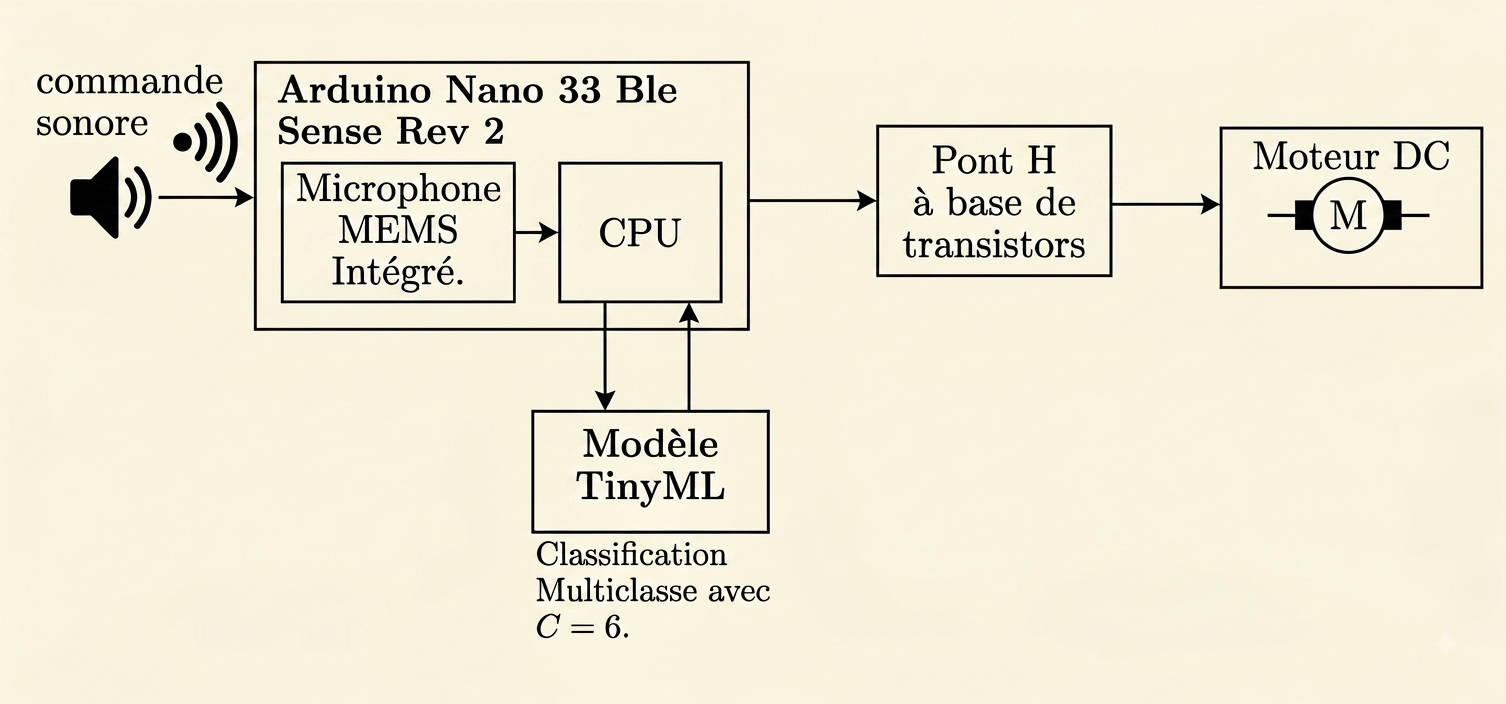
\includegraphics[width=0.8\textwidth]{./images/schema_bloc_system}
	\caption{Schéma bloc du système de commande vocal}
	\label{fig:schema_bloc1}
\end{figure}

Ce système est scindé en sous-systèmes suivants : le modèle d'apprentissage automatique, le microcontrôleur Arduino, le circuit de commande du moteur, le moteur \ac{DC} lui-même ainsi que le système d'alimentation. Dans les prochains chapitres, nous analyserons plus profondément chaque sous-système. Aussi sera-t-elle faite la conception du système avec les logiciels MultiSim(pour la simulation interactive du système), LTSpice(alternative open-source à MultiSim mais pas interactif) et KiCad, un logiciel open-source de conception de \acp{PCB} (Printed Circuit Board) ; une ouverture vers la production en masse de ce projet.

À part le logiciel cité ci-dessus, nous utilisons aussi pour l'entraînement et la définition des réseaux de neurones, les frameworks tensorflow et keras, disponibles comme modules Python. Toujours avec Python, d'autres modules comme librosa, sklearn, matplotlib et numpy nous ont beaucoup servi pour l'acquisition et le pré-traitement des données utilisées pour l'entrainement, le test et la validation du modèle.
Toutes ces ressources seront explorées afin d'aider le lecteur à mieux comprendre le travail.

Les prochains chapitres sont organisés de la façon suivante~:
\begin{itemize}
	\item le \textbf{chapitre deux} concerne la présentation du microcontrôleur : définitions, types des microcontrôleurs ainsi que les propriétés de la carte que nous avons choisi. Arduino Nano 33 \ac{BLE} Sense Rev2 est de façon large une carte composée de neuf capteurs intégrés dont un microphone, qui nous servira pour enregistrer les commandes vocales de l'opérateur. Aussi existe-t-il une grande communauté de développement des modèles \ac{ML} autour de ce microcontrôleur ;
	
	\item le \textbf{chapitre trois} est une introduction à quelques notions importantes du « machine learning » en général et du « deep learning » en particulier. La tâche que nous voulons réaliser, reconnaître des mots clés, est ce qu'on appelle un problème de classification multiclasse en machine learning, un problème quasiment impossible à résoudre en utilisant la programmation « traditionnelle » que nous connaissons. Ainsi, nous recourons aux méthodes d'apprentissage automatique dont l'usage des « réseaux de neurones ». Nous donnons dans ce chapitre les définitions et les lois qui régissent cette nouvelle façon de programmer. Nous finissons le chapitre par la conception de nos réseaux de neurones de reconnaissance vocale ;
	
	\item le \textbf{chapitre quatre} concerne l'analyse du moteur \ac{DC} à aimant permanent. Il s'agit d'un moteur à balais de la société Mabuchi que nous avons récupéré dans une ancienne radio cassette et dont nous avons téléchargé la fiche technique afin de connaître ses caractéristiques électriques. Étant donné qu'il est vieux comme moteur, tenant compte du phénomène de vieillissement, nous avons aussi fait des essais au laboratoire d'électronique de la faculté afin de connaître ses performances actuelles. Grâce à ses mesures, nous avons modélisé le moteur sur LTSpice comme la mise en série d'une résistance, d'une inductance et d'une source de tension ;
	
	\item le \textbf{chapitre cinq} concerne la conception du circuit de commande du moteur \ac{DC} et le code arduino qui doit faire tourner le modèle et interpréter ses prédictions pour le pilotage. Comme nous ne pouvons pas directement connecter le moteur à la carte arduino (pour des raisons que nous verrons), le circuit de commande en pont en H, formé de transistors bipolaires et des transistors à effet de champs, nous permettra de le faire. Il nous permettra aussi d'inverser le sens de rotation du moteur en inversant la polarité de son alimentation (le circuit d'excitation est déjà fixé, c'est un aimant permanent).
	
	\item les \textbf{tests} que nous avons réalisés sur le système sont présentés au \textbf{chapitre six} de ce rapport.
	
	\item le \textbf{chapitre sept} est la conclusion qui part d'un résumé et s'achève par des suggestions et constats ;
	\item aux \textbf{annexes}, nous mentionnons les codes que nous avons utilisés, les modules Python qui ont servi à réaliser le modèle d'apprentissage automatique.
\end{itemize}

Soulignons pour finir ce chapitre l'aide immense de l'\ac{IA} dans la réalisation de ce projet. En effet, la grande partie d'images d'illustration présentées dans ce rapport a été générée en utilisant les compétences de \textbf{Google Gemini} et \textbf{ChatGpt}. Le schéma ci-dessus par exemple, a été généré par Gemini à partir d'un schéma que nous avons fait à la main. \textbf{Claude AI} nous a beaucoup servi lors de la recherche des documents de références supplémentaires ainsi que pour comprendre le fonctionnement de l'exemple \textbf{micro-speech} de tensorflow, en partant de la mise au point du modèle \ac{ML} à son intégration dans la carte arduino ; l'acquisition d'outils comme librosa et sklearn a été largement rendu simple.

\chapter{Présentation du microcontrôleur}

\section{Le microcontrôleur}

\begin{defi}[Microcontrôleur]
	Une unité de microcontrôleur est, en général, un petit ordinateur sur une puce unique. Il est conçu et optimisé pour gérer des tâches spécifiques au sein d'un système embarqué sans nécessiter de système d'exploitation complexe, et en général sa consommation énergétique est très modeste.~\cite{ibm_microcontroller}.
\end{defi}

Une carte de microcontrôleur est un circuit imprimé formé de ce \ac{IC} compact qu'est le microcontrôleur, ainsi que d'autres composants qui interagissent. En général, quand on parle de microcontrôleur, on vise toute la carte, c'est-à-dire tout le circuit imprimé.

Les principaux composants d'un microcontrôleur sont~:
\begin{itemize}
	\item un \ac{CPU}~: c'est le composant principal, responsable de l'exécution des instructions et du contrôle des opérations~;
	\begin{figure}[H]
		\centering 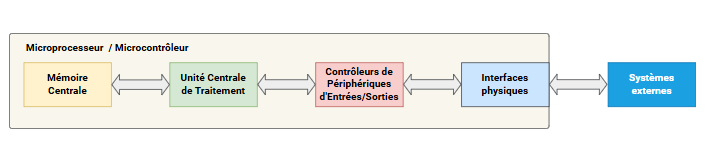
\includegraphics[width=0.7\textwidth]{./images/architecture.png}
		\caption{Architecture d'un microcontrôleur~\cite{archi_microcontroleur}}
		\label{fig:architecture_microcontrôleur}
	\end{figure}
	
	\item une \ac{RAM} et une mémoire flash non volatile pour stocker le jeu d'instructions de programmation du microcontrôleur~;
	
	\item les périphériques~: en fonction de l'application envisagée, il peut contenir divers composants auxiliaires.
\end{itemize}

\subsection{Types de microcontrôleurs}

Voici quelques-uns des types de microcontrôleurs les plus courants~:

\begin{itemize}
	\item \textbf{Microcontrôleurs 8 bits}~: type de microcontrôleur le plus élémentaire, doté d'un traitement et d'une mémoire limités, généralement utilisé dans les petits appareils tels que les jouets.
	
	\begin{figure}[H]
		\centering 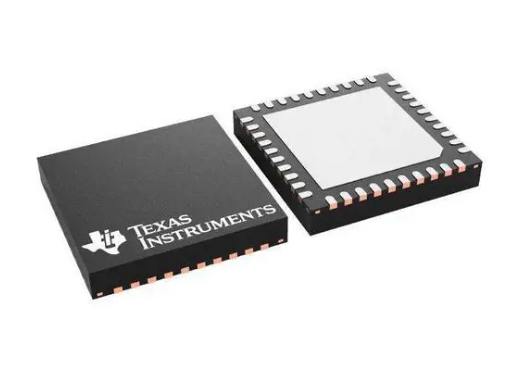
\includegraphics[width=0.6\textwidth]{./images/micro_8bits_CC2541.png}
		\caption{Microcontrôleur 8 bits CC2541 (TI)~\cite{microcontroleur8bits}}
		\label{fig:microcontrôleur8bits}
	\end{figure}
	
	\item \textbf{Microcontrôleurs 16 bits}~: deux fois plus performants que les modèles 8 bits, ils sont utilisés pour des applications plus complexes~: dispositifs médicaux, systèmes automobiles et systèmes de contrôle industriel.
	\begin{figure}[H]
		\centering 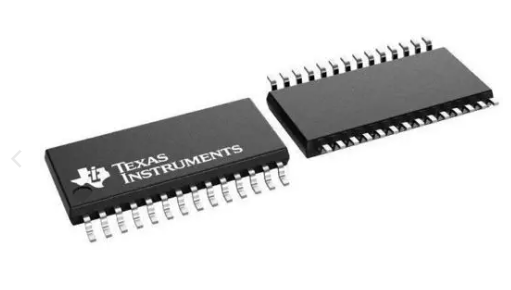
\includegraphics[width=0.6\textwidth]{./images/micro_16bits_MSP430G2553.png}
		\caption{Microcontrôleur 16 bits MSP430G2553 (TI)~\cite{microcontroleur16bits}}
		\label{fig:microcontrôleur16bits}
	\end{figure}
	
	\item \textbf{Microcontrôleurs 32 bits}~: il s'agit du type le plus puissant et le plus riche en fonctionnalités, utilisé pour des applications exigeantes, telles que les consoles de jeu et l'automatisation industrielle.
	
	\item \textbf{Microcontrôleurs \ac{RISC}}~: ils intègrent une architecture de conception qui simplifie et améliore les opérations en exécutant moins d'instructions de calcul plus rapidement que d'autres méthodologies.
	
	\item \textbf{Microcontrôleurs \ac{ARM}}~: ils intègrent l'architecture \ac{ARM} qui renforce les performances et la fiabilité. Ils sont très utilisés dans les appareils mobiles, les systèmes automobiles et les systèmes de contrôle industriels.
	
	\item \textbf{Microcontrôleurs basés sur \ac{FPGA}}~: couramment utilisés dans les applications qui nécessitent le traitement de signaux numériques, le traitement vidéo et les réseaux haut débit, ils utilisent des réseaux de portes programmables in situ (\ac{FPGA}), qui peuvent être configurés et reconfigurés au niveau matériel.
\end{itemize}

Pour ce projet, nous utilisons un Arduino Nano 33 \ac{BLE} Sense Rev2, que nous présentons dans la section suivante.

\section{Arduino Nano 33 BLE Sense Rev2}
\begin{figure}[H]
	\centering 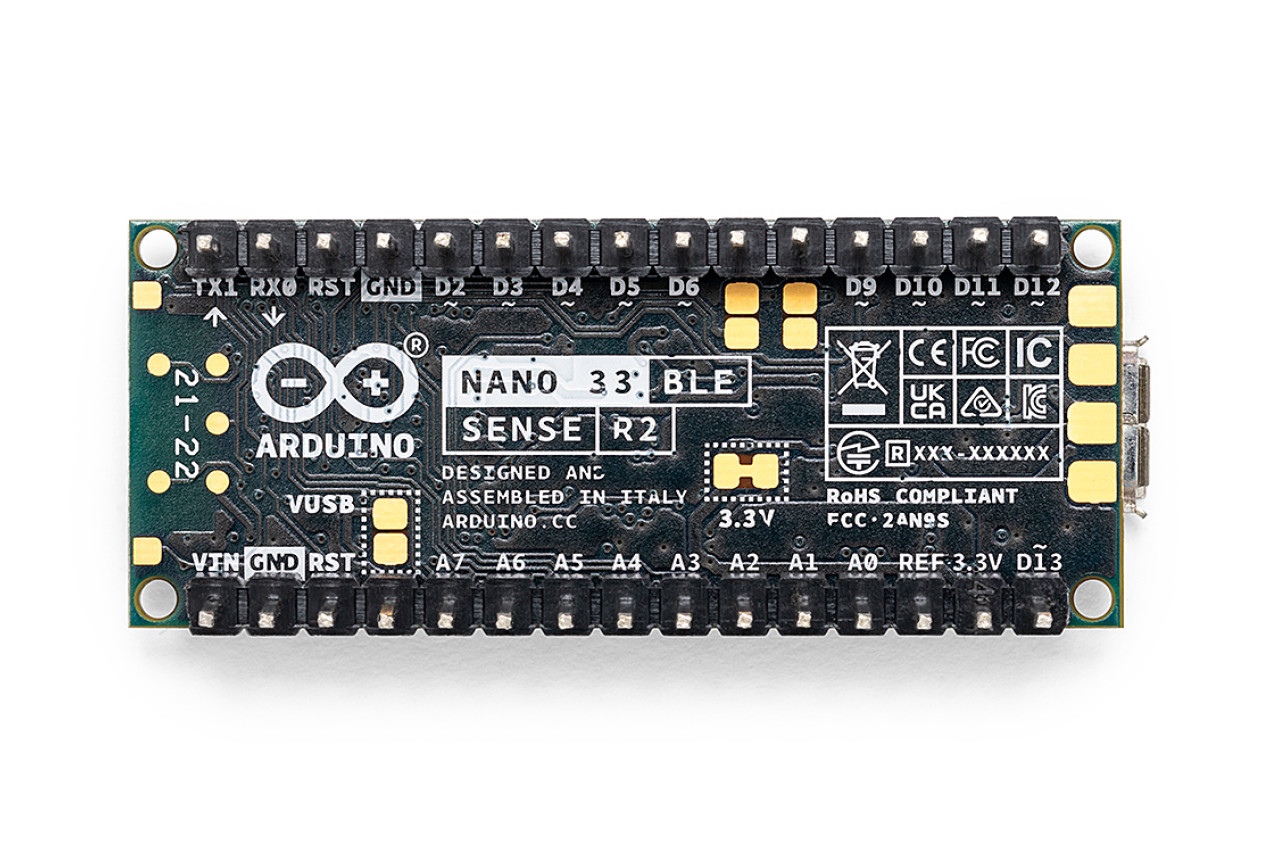
\includegraphics[width=0.5\textwidth]{./images/arduino_nano_33_ble_sense_rev2.jpg}
	\caption{Arduino Nano 33 BLE Sense Rev 2 (sans capteurs ni puce)~\cite{arduino_nano33ble}}
	\label{fig:arduinoNano33BleSenseRev2A}
\end{figure}

\begin{figure}[H]
	\centering 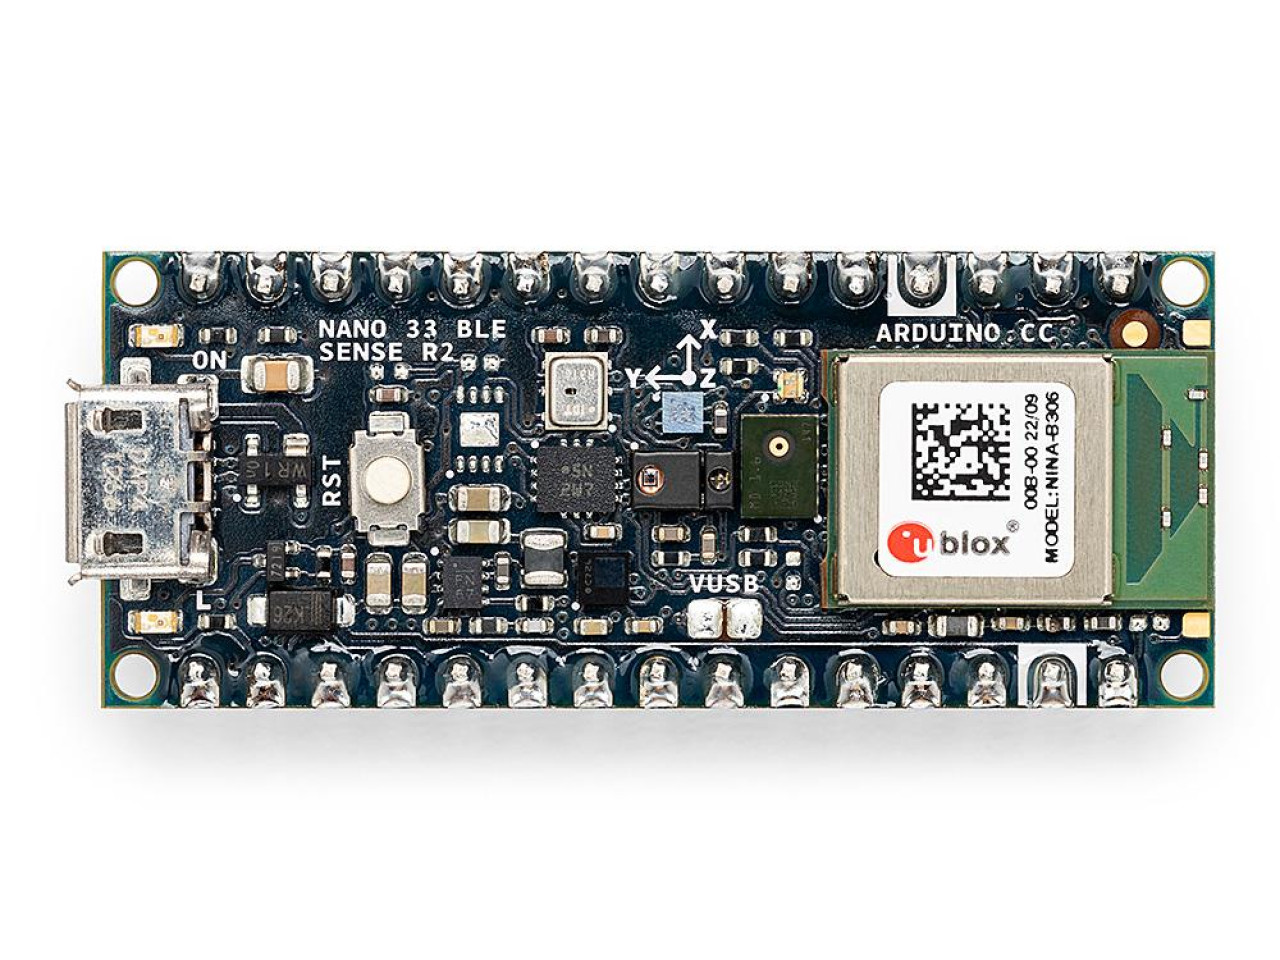
\includegraphics[width=0.7\textwidth]{./images/arduino_nano_33_ble_sense_rev2_2}
	\caption{Arduino Nano 33 BLE Sense Rev 2~\cite{arduino_nano33ble}}
	\label{fig:arduinoNano33BleSenseRev2B}
\end{figure}

Arduino est la marque d'une plateforme open-source de prototypage électronique fondée en 2005 au Politecnico di Ivrea, en Italie. La carte intègre un micro-contrôleur programmable, accessible via un \ac{IDE} simplifié basé sur le langage C/C++.

Arduino Nano 33 \ac{BLE} Sense est une carte de développement de format compact~\cite{arduino_nano33ble_manual} (\SI{45}{\milli\meter} $\times$ \SI{18}{\milli\meter}) qui se distingue de la version « Nano 33 \ac{BLE} » de base par l'ajout de neuf capteurs intégrés, dont un microphone numérique.

Voici les caractéristiques de son microprocesseur~:
\begin{itemize}
	\item \textbf{Architecture \ac{CPU}}~: \ac{ARM} Cortex-M4F (32 bits avec \ac{FPU})~\cite{arm_cortex_m4}. C'est un processeur basse consommation, caractérisé par un faible nombre de portes logiques, une faible latence d'interruption et un débogage économique.
	
	\item \textbf{Fréquence d'horloge}~: \SI{64}{\mega\hertz}. La fréquence d'horloge dans un microcontrôleur indique deux choses~: la vitesse d'exécution et la synchronisation. Plus la fréquence d'horloge est élevée, plus l'exécution des programmes est rapide. Tous les composants internes tirent leur cadencement de l'horloge.
	
	\item \textbf{Mémoire Flash}~: \SI{1}{\mega\byte}.
	
	\item \textbf{Mémoire \ac{RAM}}~: \SI{256}{\kilo\byte}.
	
	Nous devons veiller à ces deux dernières informations, car la taille du modèle d'apprentissage automatique doit satisfaire aux contraintes de mémoire du microcontrôleur. Il ne serait pas intéressant de disposer d'un modèle puissant qu'on ne sait charger en mémoire.
\end{itemize}

\subsection{Tension et alimentation}

Arduino Nano 33 \ac{BLE} Sense Rev2 peut être alimenté de trois façons différentes~: par le port \ac{USB}, par la broche \texttt{Vin} et par la broche \SI{3.3}{\volt}.
\begin{enumerate}
	\item Le port \ac{USB} permet de fournir une tension d'entrée stable de \SI{5}{\volt}.
	
	\item La tension d'entrée admissible à la broche \texttt{Vin} est de 5 à \SI{21}{\volt}. Le régulateur intégré convertit cette tension en \SI{3.3}{\volt} avant d'alimenter le microcontrôleur.
	
	\item Si l'on dispose d'une source de tension d'entrée stable capable de fournir \SI{3.3}{\volt}, nous pouvons la connecter directement à la broche \SI{3.3}{\volt} ; sinon la broche voire une grande partie du micro-contrôleur sera grillée.
\end{enumerate}

\subsection{Connectivité et entrées/sorties}

\begin{itemize}
	\item \textbf{Connectivité radio}~: Bluetooth 5.0, \ac{BLE}, \ac{NFC}, 802.15.4. La connectivité \ac{BLE} permet de communiquer sans fil avec un ordinateur (ou un smartphone) tout en consommant très peu d'énergie.
	
	\item \textbf{Nombre de broches \ac{GPIO}}~: 15.
	
	Ce sont des broches à usage général. Leurs fonctions sont décidées par logiciel, si elles doivent lire ou émettre un signal.
	
	\item \textbf{\ac{PWM}}~: disponible sur plusieurs broches, toutes les broches numériques (D2--D13).
	
	Le \ac{PWM} est une technique qui permet de simuler un signal analogique à partir d'un signal numérique. Au lieu de mettre une sortie à \SI{3.3}{\volt} en continu pour faire briller une \ac{LED} à fond, le \ac{PWM} va allumer et éteindre cette sortie très rapidement, un grand nombre de fois par seconde, en faisant varier le pourcentage du temps passé à l'état haut par rapport au temps passé à l'état bas~: le « rapport cyclique ».
\end{itemize}

\subsection{Capteurs embarqués}

En plus de ces caractéristiques, la carte dispose de neuf capteurs embarqués~: le microphone, le capteur de température, le gyroscope 3D, le magnétomètre 3D, le capteur de pression barométrique, le capteur de couleur et de proximité, le capteur d'humidité, les capteurs de geste.

Le microphone est fabriqué par des procédés de micro-fabrication fine et intégré (\ac{MEMS})~\cite{mp34dt05a_datasheet}. Une membrane mécanique extrêmement fine et conductrice, gravée dans du silicium, oscille et vibre sous l'action de variations de pression acoustique qui sont converties en signal électrique numérique.

Grâce à ce microphone intégré, nous n'avons plus besoin de réaliser une chaîne d'acquisition et de conditionnement du signal vocal.

\chapter{Conception du modèle deep learning}

\section{Introduction à l'apprentissage automatique}

Notre objectif peut être réduit à l'étude d'une forme d'\ac{IA} capable de fonctionner dans un microcontrôleur. Pour atteindre ce but, nous nous penchons vers un domaine en pleine croissance, le \ac{TinyML}, un terme désignant un ensemble de techniques permettant d'exécuter des d'algorithmes de \ac{ML} directement sur des micro-contrôleurs comme Arduino.

Les motifs qui nous ont poussés à choisir le \ac{ML} et le faire tourner dans un microcontrôleur sont~:
\begin{itemize}
	\item la beauté de ce paradigme, cette nouvelle façon de programmer des tâches compliquées comme le problème auquel nous sommes confrontés~;
	\item la faible consommation énergétique en comparaison avec des modèles hébergés sur des clouds consommant des watts~;
	\item le faible coût matériel et logiciel~;
	\item l'autonomie que peut avoir un modèle sur un microcontrôleur, rend le \ac{TinyML} encore plus intéressant.
\end{itemize}

Dans les prochaines sections, nous nous inspirons de quelques notions du livre « TinyML, Machine Learning with TensorFlow Lite on Arduino and Ultra-Low-Power Microcontrollers »~\cite{warden2019tinyml}, notamment de l'exemple « micro-speech » qui y est proposé, ainsi que d'un ouvrage de référence sur l'apprentissage automatique avec Keras et TensorFlow : "Deep Learning avec Keras et TensorFlow~: mise en \oe uvre et cas concrets"~\cite{geron2023deeplearning}.

\subsection{Machine Learning}

le \ac{ML} est une branche de l'informatique où l'on ne programme pas les règles explicitement. On montre des exemples à l'ordinateur et il découvre tout seul les règles. C'est une programmation implicite dont le résultat est un « fichier mathématique » appelé modèle.

\begin{defi}[Apprentissage automatique; Tom Mitchell, 1997]
	Étant donné une tâche $T$ et une mesure de performance $P$, on dit qu'un programme apprend à partir d'une expérience $E$ si les résultats obtenus sur $T$, mesurés par $P$, s'améliore avec l'expérience $E$.
\end{defi}

Cette définition résume à elle seule le \ac{ML}, en citant ses éléments principaux à savoir : les données(la tâche), la fonction de coût(la mesure de performance) et l'entraînement(l'expérience). Chacun de ces éléments sera abordé dans la suite.

Notons que trois situations peuvent nous pousser à choisir une approche \ac{ML} plutôt que la programmation traditionnelle~:
\begin{enumerate}
	\item quand nous sommes face à un problème que l'on ne sait pas résoudre en formulant explicitement des règles~;
	\item quand nous sommes face à un problème que l'on sait résoudre, mais que l'on ne sait pas formaliser sous forme algorithmique la façon dont nous les résolvons~;
	\item quand nous sommes face à un problème que l'on sait résoudre, mais dont les procédures sont beaucoup trop gourmandes en ressources informatiques.
\end{enumerate}

Dans notre cas, où il nous faut reconnaître des mots-clés prononcés dans un signal vocal, personne ne sait écrire explicitement un jeu de règles permettant de résoudre ce problème pour n'importe quelle voix. Même si cela était possible, un tel code serait beaucoup trop volumineux pour être chargé en mémoire d'un microcontrôleur.

Le \ac{ML} repose sur deux piliers~:
\begin{itemize}
	\item les données~: ce sont des exemples à partir desquels l'algorithme d'apprentissage va forger le modèle~;
	\item l'algorithme d'apprentissage~: c'est l'algorithme, ou le programme informatique en particulier, que nous exécutons sur les données pour produire le modèle.
\end{itemize}

Pour une présentation plus complète des notions de \ac{ML} abordées dans ce chapitre, le lecteur pourra se référer à~\cite{azencott_ml}.

\begin{defi}[Entraînement]
	C'est l'action de faire tourner un algorithme d'apprentissage sur les données pour produire le modèle.
\end{defi}

\subsubsection{Types de problèmes}

Il y a quatre grands types de problèmes que nous pouvons résoudre grâce au \ac{ML} ; il s'agit des problèmes d'apprentissage supervisé, des problèmes d'apprentissage non supervisé, des problèmes d'apprentissage semi-supervisé et des problèmes d'apprentissage par renforcement.

\begin{defi}[Apprentissage supervisé]
	Soient $m$ observations $\{\vec{x}^{(i)}\}_{i=1,2,\ldots,m}$ décrites dans un espace $\mathcal{X}$ et leurs étiquettes $\{y^{(i)}\}$ décrites dans un espace $\mathcal{Y}$. On suppose que les étiquettes sont obtenues à partir des observations grâce à une fonction $\Phi : \mathcal{X} \to \mathcal{Y}$ fixe et inconnue telle que, pour tout $i$~:
	\[ y^{(i)} = \Phi(\vec{x}^{(i)}) + \varepsilon_i \]
	avec $\varepsilon_i$ un bruit aléatoire.
\end{defi}

L'apprentissage consiste à utiliser les données pour déterminer une fonction $f : \mathcal{X} \to \mathcal{Y}$ telle que, pour tout $\vec{x}$~:
\[ f(\vec{x}) \simeq \Phi(\vec{x}). \]

L'apprentissage supervisé, comme problème d'apprentissage, se ramène en général à un problème de classification binaire(l'ensemble $\mathcal{X}$ est alors partitionné en deux sous-ensembles, celui des éléments dont l'étiquette est $1$ par exemple; et celui des éléments dont l'étiquette est $0$), un problème de classification multiclasse (avec $\mathrm{Card}(\mathcal{Y}) > 2$), ou un problème de régression (avec $\mathcal{Y} = \mathbb{R}$). Un modèle de régression prédit une valeur numérique comme le prix d'un produit ; les modèles de classification prédisent la probabilité qu'un élément appartienne à une catégorie.

\begin{defi}[Apprentissage non supervisé]
	Soient $m$ observations $\{\vec{x}^{(i)}\}_{i=1,\ldots,m}$ décrites dans un espace $\mathcal{X}$. Il s'agit d'identifier une propriété partagée par les observations.
\end{defi}

La capacité de l'apprentissage non supervisé à découvrir des similitudes et des différences dans les informations le rend idéal pour l'exploration des données. % Tiré de ibm.com

Comme tâches principales qui conduisent à l'apprentissage non supervisé nous pouvons citer~:
\begin{enumerate}
	\item le partitionnement(ou clustering)~: il consiste à identifier des groupes dans les données. Les données non étiquetées sont regroupées en fonction de leurs similitudes ou de leurs différences.~;
	
	\item la réduction de dimensionnalité~: elle consiste à rechercher un espace $\mathcal{Z}$ de dimension plus faible que l'espace $\mathcal{X}$. Les projections $\{\vec{z}^{(i)}\}$ des données sur $\mathcal{Z}$ doivent vérifier certaines propriétés.
	
	\item l'estimation de densité~: elle consiste à estimer une loi de probabilité en supposant que le jeu de données en est un échantillon aléatoire.
	
\end{enumerate}

\begin{defi}[Apprentissage semi-supervisé]
	Il consiste à apprendre des étiquettes à partir d'un jeu de données partiellement étiqueté. Cet apprentissage combine l'apprentissage supervisé et non supervisé. Les méthodes d'apprentissage semi-supervisées sont très utiles dans les cas où il est difficile d'obtenir un volume suffisant de données étiquetées.
\end{defi}

\begin{defi}[Apprentissage par renforcement]
	Dans le cadre de l'apprentissage par renforcement, le système d'apprentissage peut interagir avec son environnement et accomplir des actions. En retour de ces actions, il obtient une récompense, qui peut être positive si l'action était un bon choix, ou négative sinon. Un système d'apprentissage par renforcement génère une stratégie qui définit la meilleure façon d'obtenir le plus de récompenses. Les applications principales de l'apprentissage par renforcement se trouvent dans la robotique et les jeux comme le go ou les échecs.
\end{defi}

\begin{figure}[H]
	\centering
	\begin{minipage}[t]{0.45\textwidth}
		\centering
		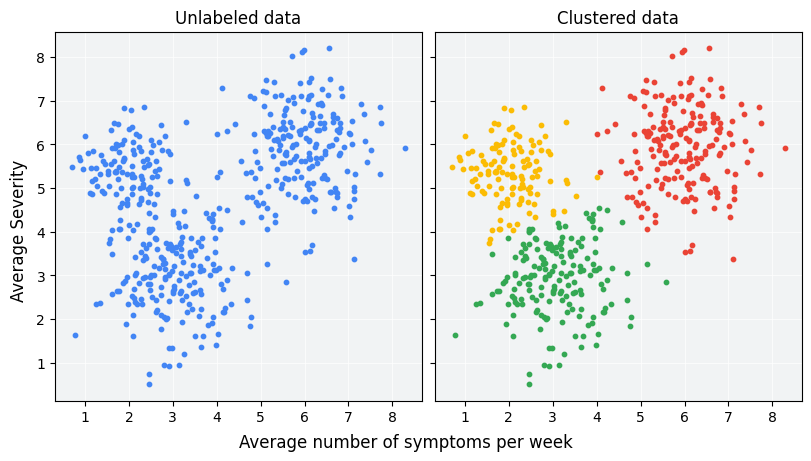
\includegraphics[width=\textwidth]{./images/clustering}
		\caption{Clustering}
		\label{fig:clustering}
	\end{minipage}
	\hfill
	\begin{minipage}[t]{0.45\textwidth}
		\centering
		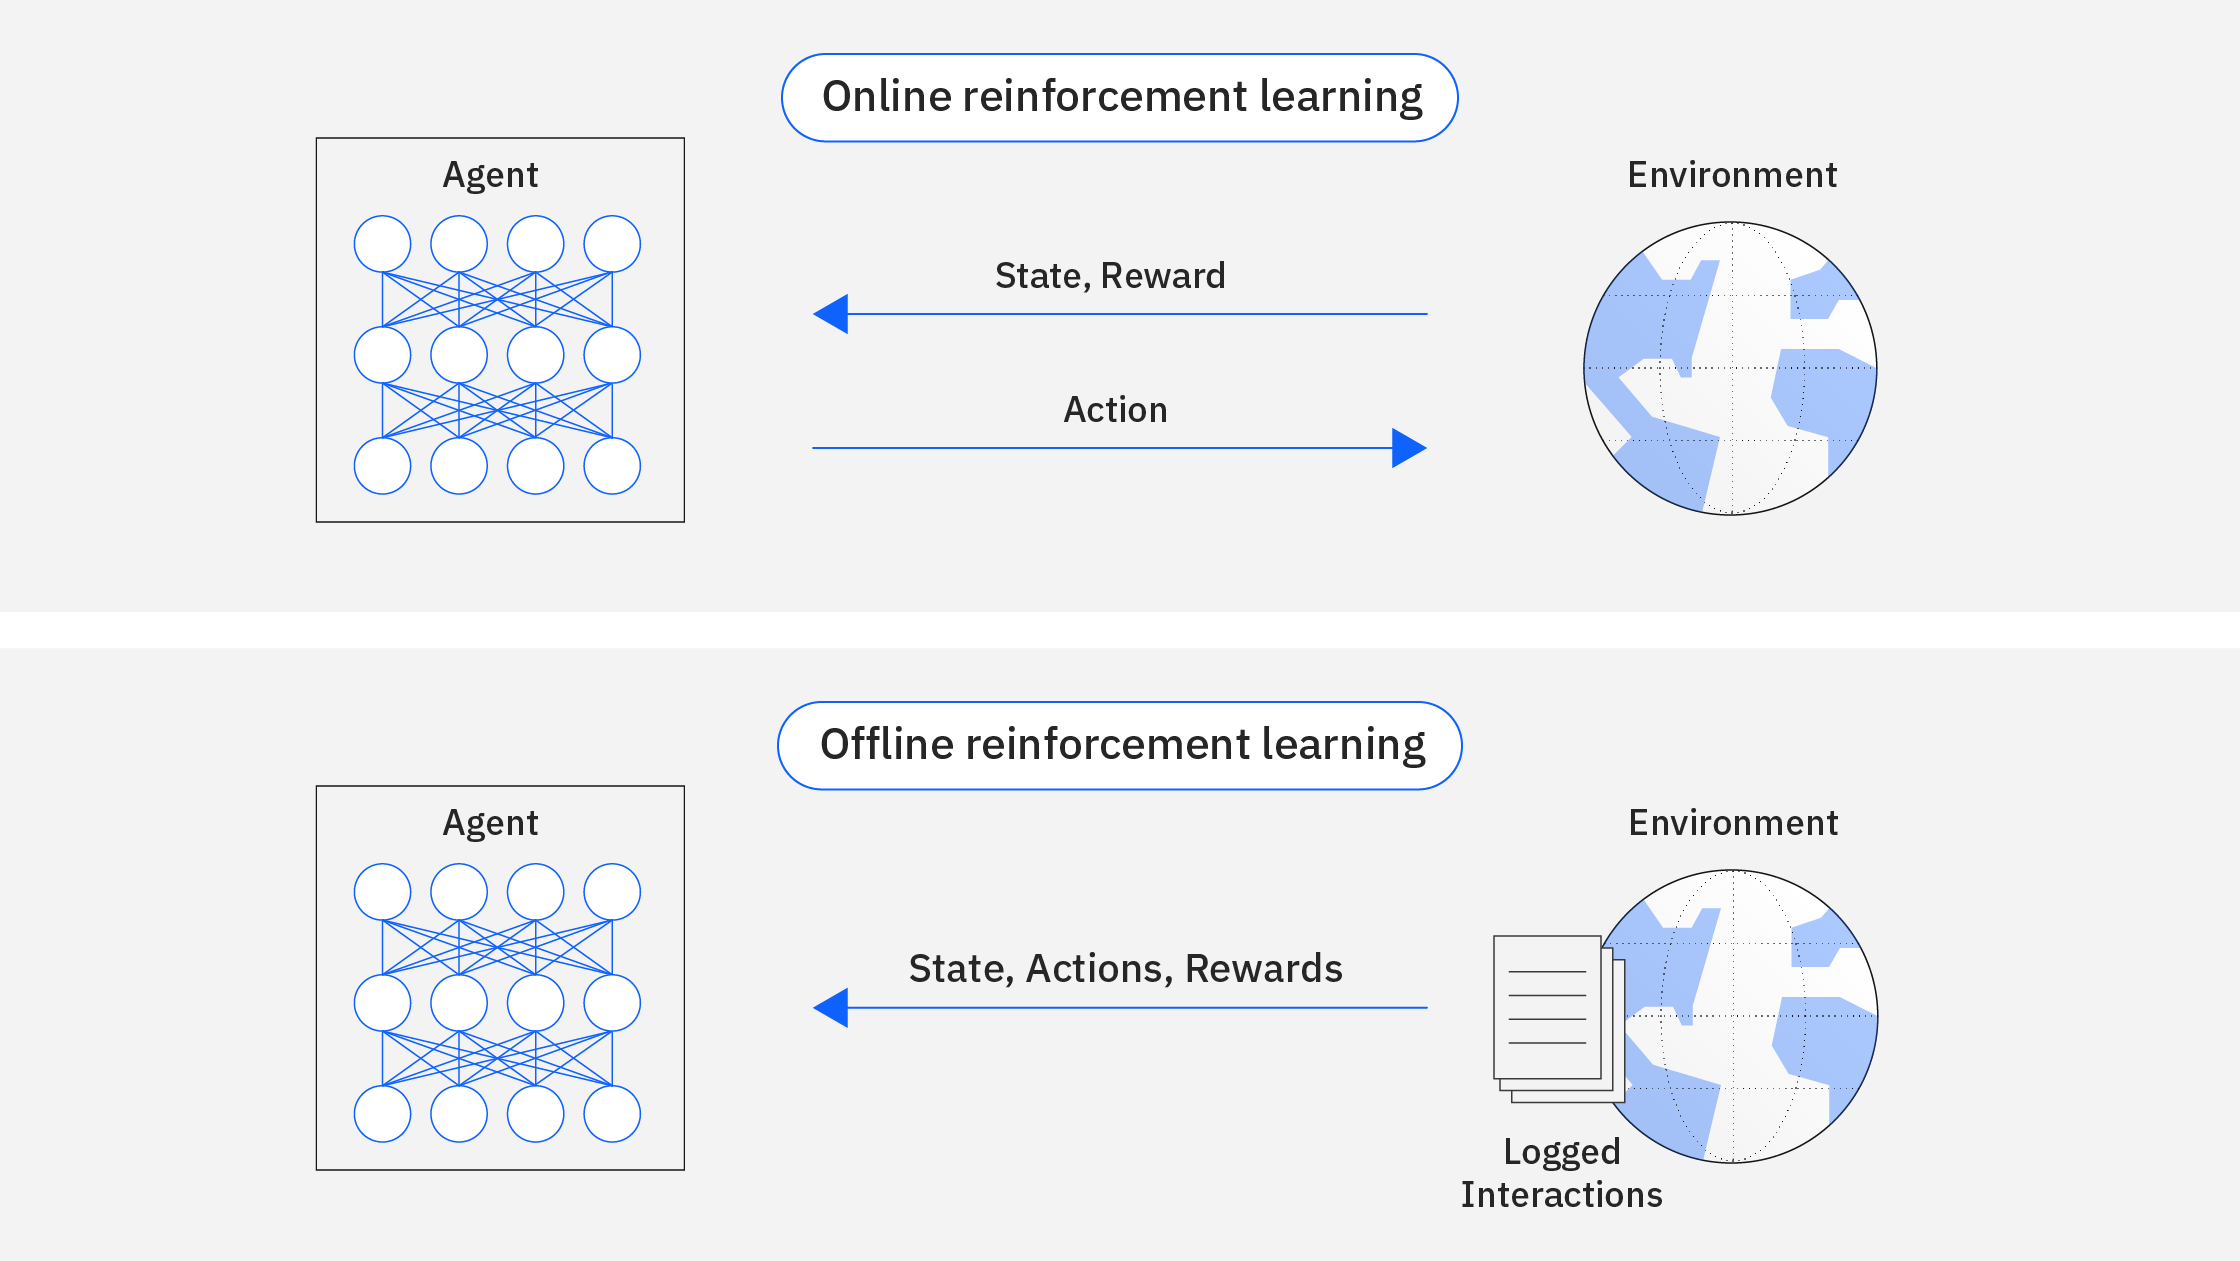
\includegraphics[width=\textwidth]{./images/renforcement}
		\caption{Renforcement}
		\label{fig:renforcement}
	\end{minipage}
	
	\vspace{0.8cm}
	
	\begin{minipage}[t]{0.45\textwidth}
		\centering
		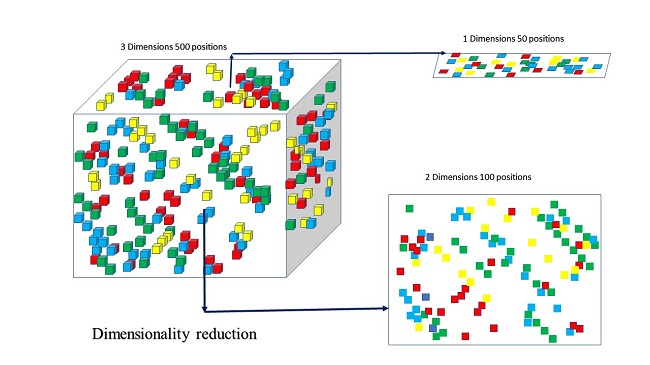
\includegraphics[width=1.2\textwidth]{./images/reduction}
		\caption{Réduction de dimension}
		\label{fig:reduction}
	\end{minipage}
	\hfill
	\begin{minipage}[t]{0.45\textwidth}
		\centering
		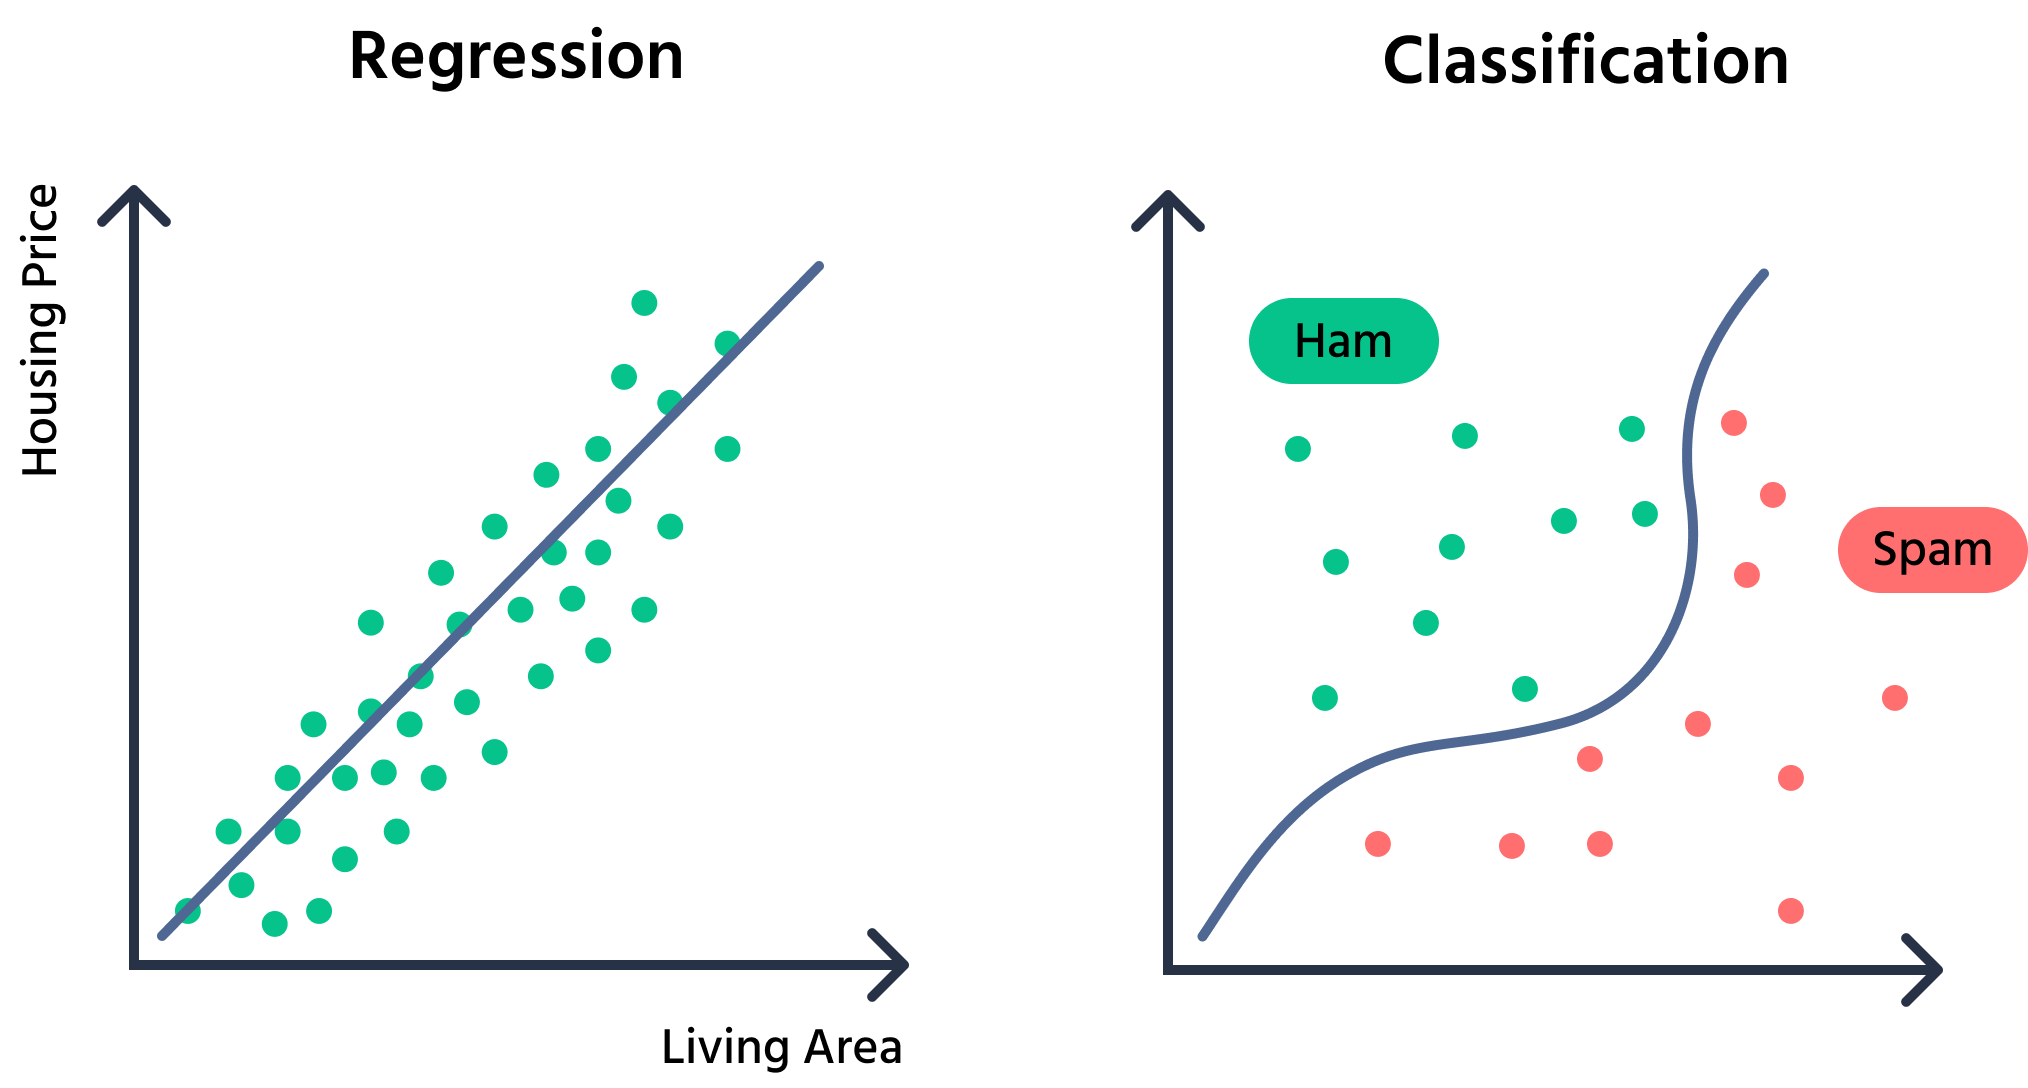
\includegraphics[width=\textwidth]{./images/regression_classification}
		\caption{Classification vs Régression}
		\label{fig:classification}
	\end{minipage}
\end{figure}
\vspace{0.8cm}

Tout système \ac{ML} passe en général par deux phases~:
\begin{enumerate}
	\item l'entraînement, phase durant laquelle, le système est entraîné sur un jeu de données dit d'entraînement~;
	\item la phase d'inférence, phase durant laquelle le système applique ce qu'il a appris sur de nouvelles données et effectue des prédictions.
\end{enumerate}

Plongeons maintenant dans l'apprentissage supervisé, car c'est le type d'apprentissage qui nous concerne.

\subsubsection{Apprentissage supervisé}

Dans de nombreuses situations, on se ramènera au cas où $\mathcal{X}=\mathbb{R}^{p}$ est l'ensemble des observations. Ainsi, chaque observation est représentée par $p$ variables.

On appelle "matrice des données" ou "matrice de design", la matrice $X \in \mathbb{R}^{n*p}$ telle que $X_{ij}=x_j^{i}$ soit la j-ème variable de la i-ème observation. Les observations sont donc les lignes de la matrice des données.

\begin{defi}[Fonction de décision]
	Dans le cadre d'un problème de classification binaire, on appelle fonction de décision ou fonction discriminante, une fonction $g : \mathcal{X} \to \mathbb{R}$ telle que $f(\vec{x})=0$ si $g(\vec{x}) \leq 0$, et $f(\vec{x})=1$ si $g(\vec{x}) > 0$.
	Dans le cas d'une classification multi-classe, on appelle fonction de décision, une fonction $g : \mathcal{X} \to \mathbb{R}$ telle que pour chaque classe $c$ des $C$ catégories, nous avons~:
	\[ f(\vec{x}) = \operatorname*{arg\,max}_{c=1,\ldots,C} g_c(\vec{x}). \]
\end{defi}

La fonction $\operatorname{arg\,max}$ renvoie l'indice $c$ tel que $g_c(\vec{x})$ soit maximale.

Les fonctions de décision nous permettent de partitionner l'espace des observations en régions de décision. Dans le cas général d'un problème de classification multi-classe, nous avons $C$ régions de décision : $R_c = \{\vec{x} \in \mathcal{X} | g_c(\vec{x}) = \operatorname*{max}_{k} g_k(\vec{x})\}$.

\begin{defi}[Frontière de décision]
	On appelle frontière de décision ou discriminant, l'ensemble des points de $\mathcal{X}$ où une fonction de décision s'annule.
\end{defi}

Une façon plus générale de voir ce problème est de considérer qu'étant donné un jeu de $n$ observations étiquetées $D=\{(\vec{x}^i, \vec{y}^i)\}$ et un espace d'hypothèses $\mathcal{F}$ décrivant les fonctions de modélisation du problème ; la tâche d'apprentissage supervisé consiste à supposer que les étiquettes $y^i$ ont été calculées grâce à une fonction $\phi : \mathcal{X} \to \mathcal{Y}$ et à trouver une hypothèse $f \in \mathcal{F}$ qui approche au mieux $\phi$. Pour y arriver, deux outils sont exploités~:

\begin{itemize}
	\item une façon de quantifier la qualité d'une hypothèse;
	\item une façon de chercher une hypothèse optimale dans $\mathcal{F}$.
\end{itemize}

\subsubsection{Fonction de coût et risque}

\begin{defi}[Fonction de coût]
	Étant donné un jeu de $m$ observations étiquetées $D = \{(\vec{x}^{(i)}, y^{(i)})\}$, on appelle fonction de coût une fonction $L : \mathcal{Y} \times \mathcal{Y} \to \mathbb{R}$, qui associe à une prédiction $f(\vec{x}^{(i)})$ et à une vraie valeur $y^{(i)}$ une valeur réelle qui symbolise la qualité de la prédiction. Elle est d'autant plus grande que l'étiquette $f(\vec{x})$ est éloigné de la vraie valeur.
\end{defi}

\begin{defi}[Risque]
	L'espérance mathématique d'une fonction de coût $R(h)$ est appelée risque~:
	\[ R(h) = \mathbb{E}_{\vec{x}} \left[ L(h(\vec{x}), y) \right] \]
	et
	\[ f(\vec{x}) = \operatorname*{arg\,min}_{h \in \mathcal{F}} \mathbb{E}_{\vec{x}} \left[ L(h(\vec{x}), y) \right]. \]
\end{defi}

\begin{defi}[Risque empirique]
	Soit $\{(\vec{x}^{(i)}, y^{(i)})\}$ un jeu de $m$ observations étiquetées, l'estimateur empirique du risque $R(h)$ est la prédiction moyenne empirique~:
	\[ R_n(h) = \frac{1}{n} \sum_{i=1}^{n} L(h(\vec{x}^{(i)}), y^{(i)}) \]
	et
	\[ f(\vec{x}) = \operatorname*{arg\,min}_{h \in \mathcal{F}} R_n(h). \]
\end{defi}

\subsection{Régression linéaire}

Un modèle de régression linéaire effectue une prédiction en calculant une somme pondérée des variables d'entrée, en y ajoutant un terme constant appelé « biais » (ou parfois « ordonnée à l'origine »)~:
\[ \hat{y} = \theta_0 + \theta_1 x_1 + \cdots + \theta_m x_m = \vec{x} \cdot \vec{\theta} \]
avec $\vec{\theta}$ le vecteur des paramètres du modèle hypothèse. Par souci d'efficacité, on réalise souvent plusieurs prédictions simultanément. Pour ce faire, on regroupe dans une même matrice $X$ toutes les observations pour lesquels on souhaite faire des prédictions.

Les vecteurs $\vec{x}$ ont tous comme premier élément le nombre $1$, pour permettre le produit scalaire avec l'ajout du biais.

\[ \hat{\vec{y}} = X \cdot \vec{\theta} \]

$\hat{\vec{y}}$ est le vecteur des prédictions du modèle. Son $i$-ème élément correspond à la $i$-ème observation. La fonction de coût la plus courante pour un modèle de régression linéaire est le \ac{RMSE}, donnée par l'expression~:
\[ \mathrm{RMSE}(X, \hat{\theta}) = \left( \frac{1}{m} \sum_{i=1}^{m} \left[ \vec{x}^{(i)} \cdot \vec{\theta} - y^{(i)} \right]^2 \right)^{1/2} \]

L'entraînement consiste à trouver la valeur de $\vec{\theta}$ qui minimise cette fonction de coût. Il existe une formule qui donne directement la valeur de $\vec{\theta}$ qui minimise \ac{RMSE}, appelée équation normale~:
\[ \hat{\vec{\theta}} = (X^{\mathrm{T}} X)^{-1} X^{\mathrm{T}} \vec{y} \]
en supposant que $X^{\mathrm{T}} X$ est inversible.

Nous remarquons la difficulté d'exécuter cette équation sur un ordinateur en terme de complexité, quand nous avons une très grosse matrice.

\begin{rem}[\textbf{Complexité de l'équation normale}]
	Pour nous en rendre compte, supposons que $X^{\mathrm{T}} X$ est inversible $(X \in \mathbb{R}^{n \times p})$. Sondons seulement deux opérations~:
	\begin{itemize}
		\item la transposée : $n \times p$ opérations;
		\item le premier produit matriciel à gauche: $x_{ij} = \sum_{k=1}^{m} X_{ik}^{\mathrm{T}} \cdot X_{kj}$; il faut $m$ produits et $(m-1)$ additions, soit $2m-1$ opérations par coefficient. Donc, pour toute la matrice, il faut $p^2 \times (2m-1)$ opérations!
	\end{itemize}
	
	Pour se faire une idée, rien que pour la première multiplication et la première transposée, si nous prenons $m=1000$ et $p=10$ : nous aurons $10000$ opérations pour la transposée et $199900$ opérations pour la multiplications. C'est à dire un total de $209900$ opérations!
\end{rem}

Cette méthode d'optimisation est limitée par la taille de la matrice des données. Le temps d'exécution est directement affecté par la taille de l'entrée.

\subsection{Descente de gradient}

\subsubsection{L'idée générale}

Il s'agit d'un algorithme d'optimisation très générique, capable de trouver des solutions à un grand nombre de problèmes. Le principe de la descente de gradient est de modifier itérativement les paramètres afin de minimiser une fonction de coût.

Cet algorithme calcule le gradient de la fonction de coût au point $\theta$ puis progresse en direction du gradient descendant. Lorsque ce gradient devient nul, c'est le minimum(local ou global). En pratique, on remplit $\vec{\theta}$ avec des valeurs aléatoires(initialisation).

\begin{defi}[Hyperparamètre]
	Paramètre d'entraînement non affecté par l'algorithme d'apprentissage(comme la descente de gradient). C'est une variable de configuration définie en amont pour gérer l'entraînement d'un modèle d'apprentissage automatique.
\end{defi}

Pour les \ac{NN}, que nous aborderons dans les prochaines sections, les hyperparamètres sont \textbf{le taux d'apprentissage, la décroissance du taux d'apprentissage, la taille du lot, le nombre de couches cachées, le nombre de neurones par couches, les époques et la fonction d'activation}.

Le taux d'apprentissage(learning rate) est un hyperparamètre qui indique le pas avec lequel nous approchons un minimum. Si il est trop petit, l'algorithme devra effectuer un grand nombre d'itérations pour converger ; trop grand, on risque de dépasser le minimum.

Dans le jargon des réseaux de neurones, la taille du lot désigne le nombre d'échantillons que le modèle traitera avant de mettre à jour ses paramètres. A elle seule, une taille de lot trop importante dégrade les performances globales ; mais ajuster en même temps que le taux d'apprentissage, elle permet d'atténuer cette perte.

\begin{figure}[H]
	\centering
	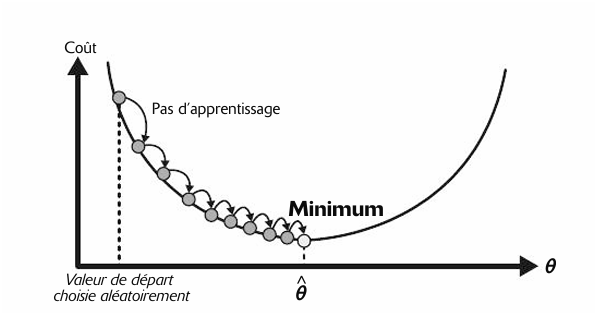
\includegraphics{./images/descenteGradient}
	\caption{Descente de gradient}
	\label{fig:gradient_descent}
\end{figure}

Notons que le réglage des hyperparamètres est crucial car il détermine la structure, l'efficacité de l'entraînement et les performances d'un modèle. L'objectif du réglage est d'équilibrer le compromis \textbf{biais-variance}. Le biais correspond à l'écart entre les prédictions du modèle et la réalité. La variance représente la sensibilité d'un modèle aux nouvelles données. Les modèles à faible biais sont précis, tandis que ceux à faible variance sont cohérents.

Lorsqu'on effectue une descente de gradient, on doit veiller à ce que toutes les variables aient la même échelle, sinon la convergence sera beaucoup plus lente. Pour cela, il faudrait normaliser les données. Une façon de le faire de centrer et réduire les variables d'entrées.

\subsubsection{Types de descente de gradient}

\paragraph{a. Descente de gradient ordinaire}

Avec
\[ \nabla_\theta \mathrm{MSE}(\vec{\theta}) = \frac{2}{m} \sum_{i=1}^{m} (\vec{\theta} \cdot \vec{x}^{(i)} - y^{(i)}) x_j^{(i)} = \frac{2}{m} X^{\mathrm{T}} (X \cdot \vec{\theta} - \vec{y}) \]
et
\[ \vec{\theta}^{(\text{étape suivante})} = \vec{\theta} - \eta \cdot \nabla_\theta \mathrm{MSE}(\vec{\theta}) \]
où $\eta$ est le taux d'apprentissage et $\mathrm{MSE}$(Mean Square Error) l'erreur quadratique moyenne est la fonction de coût à optimiser.

Chacune des itérations sur le jeu de données d'entraînement s'appelle "époque". Si les données sont normalisées, un taux d'entraînement de $0.01$ sera souvent correct. Il faut choisir un très grand nombre d'époques, mais interrompre l'algorithme lorsque la norme du vecteur gradient devient inférieure à un très petit nombre $\epsilon$ appelé "tolérance".

\paragraph{b. Descente de gradient stochastique}

Elle consiste à choisir aléatoirement une observation au hasard dans le jeu de données d'entraînement à chaque étape et calculer les gradients en se basant sur cette seule observation. Elle a plus de chance de trouver le minimum global que la descente de gradient ordinaire.

\paragraph{c. Descente de gradient par mini-lots}

A chaque itération, au lieu de calculer les dérivées partielles sur l'ensemble du jeu des données d'entraînement ou sur une seule observation, la descente de gradient par mini-lots calcule le gradient sur de petits sous-ensembles d'observations sélectionnées aléatoirement qu'on appelle "mini-lots".

\subsection{Régression polynomiale}

Si la complexité des données ne peut se réduire par une droite, on peut ajouter les puissances de chacune des variables comme nouvelles variables, puis entraîner un modèle linéaire sur ce nouvel ensemble de variables. Cette technique est appelée régression polynomiale, avec un modèle liant $y$ aux variables $x$ suivant l'expression polynomiale de degré $d$ suivant~:
\[ y = \beta_0 + \beta_1 x + \beta_2 x^2 + \cdots + \beta_d x^d + \varepsilon. \]

On note que le modèle reste linéaire pour les coefficients $\beta_i$. On peut donc l'estimer par les méthodes montrées précédemment.

\subsection{Courbes d'apprentissage}

Les courbes d'apprentissage représentent graphiquement l'évolution des performances du modèle(l'erreur d'entraînement et l'erreur de validation) en fonction des itérations(époques). On évalue le modèle en calculant les erreurs en utilisant à la fois le jeu de données d'entraînement et le jeu de validation.

\begin{defi}[Généralisation]
	On appelle généralisation la capacité d'un modèle à faire des prédictions correctes sur de nouvelles données, qui n'ont pas été utilisées pour le construire.
\end{defi}

\begin{defi}[Sur-apprentissage]
	On dit d'un modèle qui, plutôt que de capturer la nature des objets à étiqueter, modélise aussi le bruit et n'est pas en mesure de généraliser, qu'il sur-apprend ou sur-ajuste.
\end{defi}

\begin{defi}[Sous-apprentissage]
	On dit d'un modèle qui est trop simple pour avoir de bonnes performances même sur les données utilisées pour le construire, qu'il sous-apprend ou sous-ajuste.
\end{defi}

Pour limiter le risque de sur-apprentissage, il est donc souhaitable de limiter la complexité du modèle, car plus un modèle est complexe, plus il a de chances de sur-apprendre.

Pour un modèle qui sous-ajuste, les deux courbes d'apprentissage atteignent un plateau, elles sont proches et relativement hautes. Pour un modèle qui sur-ajuste, le modèle donne des résultats nettement meilleurs sur le jeu d'entraînement que sur le jeu de validation.

Un moyen de réduire le sur-ajustement consiste à « régulariser » le modèle, c'est-à-dire à lui imposer des contraintes. Pour un modèle linéaire, la régularisation consiste en général à imposer des contraintes aux coefficients de pondération du modèle.

\begin{figure}[H]
	\centering
	\begin{minipage}[t]{0.45\textwidth}
		\centering
		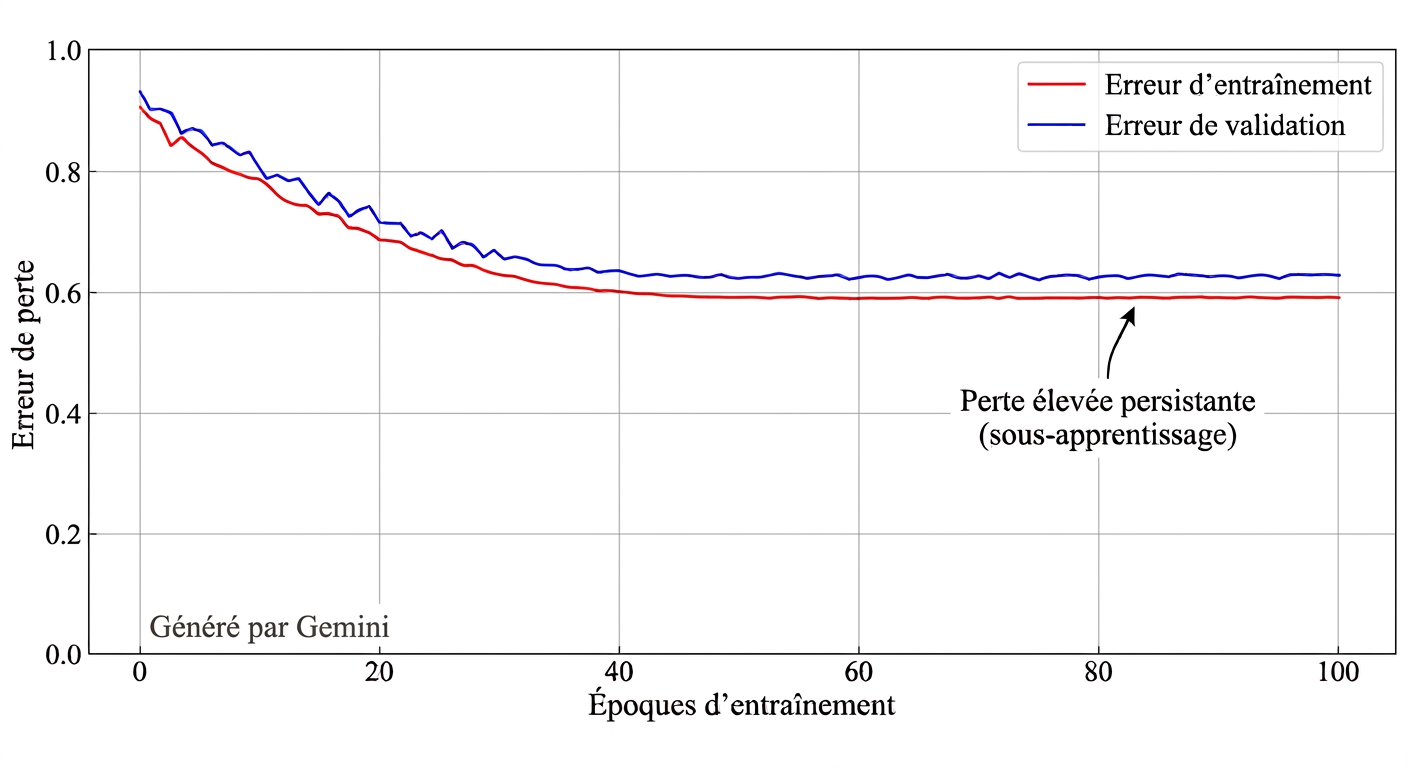
\includegraphics[width=\textwidth]{./images/sous-apprentissage}
		\caption{Le sous-apprentissage}
		\label{fig:sousapprentissage}
	\end{minipage}
	\hfill
	\begin{minipage}[t]{0.45\textwidth}
		\centering
		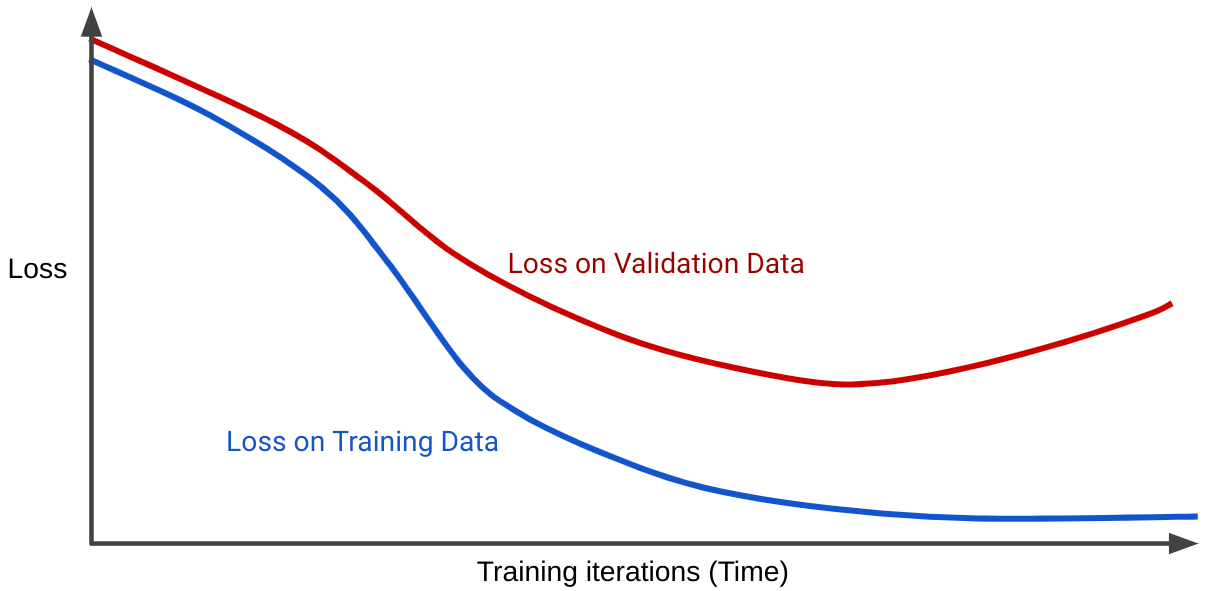
\includegraphics[width=\textwidth]{./images/sur-apprentissage}
		\caption{Le sur-apprentissage}
		\label{fig:surapprentissage}
	\end{minipage}
\end{figure}

\begin{defi}[\textbf{Arrêt précoce}(Early Stopping)]
	Une manière de régulariser les algorithmes d'apprentissage itératifs consiste à stopper l'apprentissage dès que l'erreur de validation atteint un minimum.
\end{defi}

L'arrêt précoce nous sera très utile lors de l'entraînement de notre modèle de classification que nous réaliserons avec "keras".

\subsection{Régression logistique}

Certains algorithmes de régression peuvent être utilisés pour la classification (et inversement). La régression logistique est utilisée pour estimer la probabilité qu'une observation appartienne à une classe particulière. Si la probabilité estimée est supérieure à un seuil donné, alors le modèle prédit que l'observation appartient à cette classe (classe positive), sinon c'est l'autre classe (classe négative).

$\hat{p} = h_\theta(\vec{x}) = \sigma(\vec{\theta} \cdot \vec{x})$ est la probabilité estimée par le modèle de régression logistique. La fonction $\sigma$ est une fonction sigmoïde qui renvoie des valeurs comprises entre $0$ et $1$~:
\[ \sigma(t) = \frac{1}{1 + \exp(-t)} \]

La prédiction du modèle de régression logistique est alors~:
\[ \hat{y} = \begin{cases} 0 & \text{si } \hat{p} < 0{,}5 \\ 1 & \text{si } \hat{p} \geq 0{,}5 \end{cases} \]

Pour une seule observation d'entraînement, la fonction de coût est donnée par~:
\[ c(\vec{\theta}) = \begin{cases} -\log(\hat{p}) & \text{si } y = 1 \\ -\log(1-\hat{p}) & \text{si } y = 0 \end{cases} \]

Pour $m$ observations, nous avons~:
\[ J(\vec{\theta}) = -\frac{1}{m} \sum_{i=1}^{m} \left[ y^{(i)} \log(\hat{p}^{(i)}) + (1-y^{(i)}) \log(1-\hat{p}^{(i)}) \right] \]
qu'on appelle aussi « perte logistique ». Et~:
\[ \frac{\partial}{\partial \theta_j} J(\vec{\theta}) = \frac{1}{m} \sum_{i=1}^{m} \left[ \sigma(\vec{\theta}^{\mathrm{T}} \vec{x}^{(i)}) - y^{(i)} \right] x_j^{(i)} \]

Pour avoir un classificateur pour plus de deux classes, on entraîne un classificateur binaire pour chaque classe (approche une-contre-toutes). Une autre approche, la régression softmax, est capable de traiter plusieurs classes simultanément. Étant donné une observation $\vec{x}$, le modèle softmax calcule d'abord un score $s_k(\vec{x})$ pour chaque classe $k$, puis on estime la probabilité de chaque classe en appliquant aux scores la fonction softmax.

\[ s_k(\vec{x}) = \vec{\theta}^{(k)} \cdot \vec{x} \]
où chaque classe possède son propre vecteur de paramètres $\vec{\theta}^{(k)}$. Ils constituent les lignes de la matrice de paramètres $\Theta$.

\[ \hat{p}_k = \sigma(s(\vec{x}))_k = \frac{\exp(s_k(\vec{x}))}{\sum_{j=1}^{K} \exp(s_j(\vec{x}))} \]

$K$ étant le nombre de classes et $s(\vec{x})$ un vecteur des scores de chaque classe.

\[ \hat{y} = \operatorname*{arg\,max}_k \sigma(s(\vec{x}))_k = \operatorname*{arg\,max}_k s_k(\vec{x}). \]

Pour l'entraînement, on définit la fonction de coût appelée « entropie croisée »~:
\[ J(\Theta) = -\frac{1}{m} \sum_{i=1,m} \sum_{k=1,K} y_k^{(i)} \log(\hat{p}_k^{(i)}) \]
et
\[ \nabla_{\theta^{(k)}} J(\Theta) = \frac{1}{m} \sum_{i=1,m} \left( \hat{p}_k^{(i)} - y_k^{(i)} \right) \vec{x}^{(i)}. \]

\section[Réseaux de neurones avec Keras]{Introduction aux réseaux de neurones artificiels avec Keras}

Les réseaux de neurones artificiels existent déjà depuis un bon moment. Ils ont été décrits pour la première fois en 1943 par le neurophysiologiste Warren McCulloch et le mathématicien Walter Pitts. L'intérêt pour l'étude des réseaux de neurones (le connexionnisme) a repris surface au début des années 1980 avec l'avènement de nouvelles techniques d'apprentissage et de nouvelles architectures.

\subsection{Le perceptron}

Inventé en 1957 par Frank Rosenblatt, c'est une architecture de réseau de neurones artificiels très simple, basée sur un neurone appelé « \ac{ULS} » ou unité linéaire à seuil. Les entrées et la sortie sont des nombres et chaque connexion en entrée possède un « poids ». La \ac{ULS} calcule une somme pondérée des entrées puis elle applique une fonction échelon à cette somme et produit le résultat~:
\[ h_{\vec{w}}(\vec{x}) = \mathrm{step}(z) = \mathrm{step}(\vec{w} \cdot \vec{x}) \]
avec $\vec{w}$ un vecteur colonne des poids.

Un perceptron est constitué d'une ou plusieurs \ac{ULS} organisées en une seule couche, chaque \ac{ULS} étant connectée à toutes les entrées. C'est ce qu'on appelle couche « dense » ou « intégralement connectée ».

\begin{figure}[H]
	\centering
	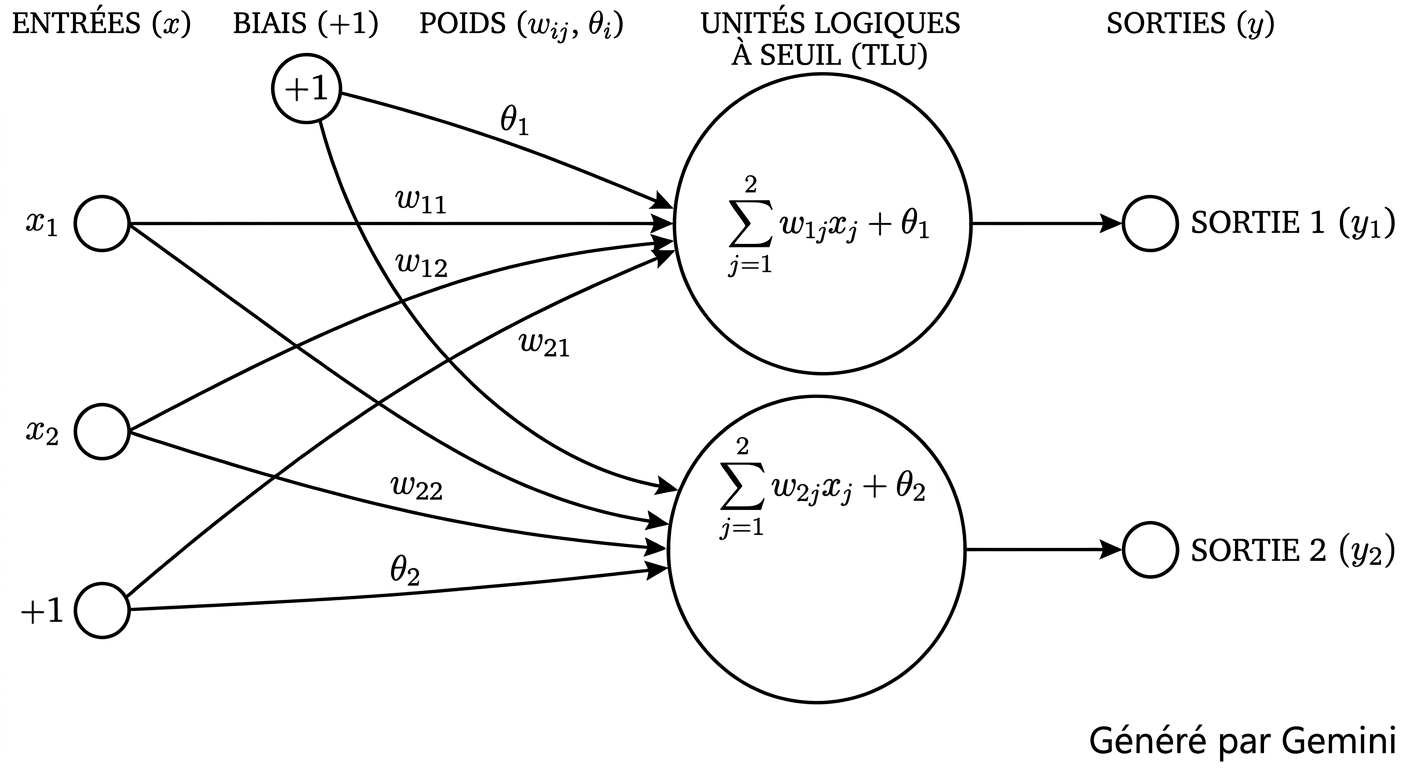
\includegraphics{./images/perceptron}
	\caption{Perceptron à deux \acp{ULS}}
	\label{fig:perceptron}
\end{figure}

Le vecteur de sortie d'une couche dense est calculé comme~:
\[ \vec{h}_{W,\vec{b}} = \vec{\Phi}(X^{\mathrm{T}} W + \vec{b}) \]
avec $X$ la matrice des données où une ligne est une observation, $W$ la matrice des poids, une ligne par entrée et une colonne par neurone, $\vec{b}$ le vecteur des termes constants, un terme par neurone, et $\Phi$ la fonction d'activation.

En mathématiques, on ne peut effectuer la somme d'une matrice et d'un vecteur. Cependant, dans le domaine de l'analyse de données, on autorise la diffusion automatique, le broadcasting, qui consiste à ajouter le vecteur à chacune des lignes de la matrice.

La règle d'apprentissage du perceptron renforce les connexions qui aident à réduire l'erreur~:
\[ W_{i,j}^{(\text{étape suivante})} = W_{i,j} + \eta (y_i - \hat{y}_i) x_i \]

Un perceptron multicouche est constitué d'une couche d'entrée, d'une ou plusieurs couches de \ac{ULS} appelées « couches cachées » et d'une dernière couche de \ac{ULS} appelée « couche de sortie ». L'entraînement d'un perceptron multicouche se fait par la méthode de « \textbf{rétro-propagation} ».

\begin{defi}[fonction d'activation]
	Il s'agit d'une fonction mathématique qui détermine la sortie d'un neurone en fonction d'un ensemble d'entrées. Elle décide si un neurone doit être actif ou inactif et introduit la non-linéarité, permettant à un \ac{DNN} d'apprendre de structures complexes.
\end{defi}
Sans une fonction d'activation, le réseau de neurones se comporterait comme un modèle de régression linéaire simple, incapable de saisir des motifs complexes quelle que soit sa profondeur. Les fonctions d'activation couramment utilisées sont~:

\begin{itemize}
	\item \textbf{Sigmoïde} : transforme tout nombre réel dans l'intervalle de 0 à 1.
	\item \textbf{\ac{ReLU}} : produit 0 pour les valeurs négatives et conserve les valeurs positives inchangées.
	\item \textbf{Tanh} : similaire à la fonction sigmoïde mais produit des valeurs entre $-1$ et 1.
\end{itemize}

\subsection{L'algorithme de rétro-propagation}

Voici les six étapes principales de l'algorithme de rétro-propagation tel que présenté dans le livre \textbf{A. Géron}\cite{geron2023deeplearning}~:
\begin{enumerate}
	\item il traite un mini-lot à la fois (par exemple 32 instances) et parcourt le jeu d'entraînement complet plusieurs fois (autant de fois qu'il y a d'époques)~;
	\item chaque mini-lot est transmis à la couche d'entrée du réseau, qui l'envoie à la première couche cachée~; le résultat de cette couche est calculé et transmis à la couche suivante, et ainsi de suite jusqu'à la couche de sortie~: c'est la « passe en avant », tous les résultats intermédiaires sont conservés puisqu'ils sont nécessaires pour la passe en arrière~;
	\item l'algorithme mesure l'erreur de sortie du réseau, c'est-à-dire l'écart entre la sortie obtenue et la sortie voulue, à l'aide d'une fonction de coût~;
	\item il calcule ensuite dans quelle mesure chaque connexion de la dernière couche cachée a contribué à cette erreur, en appliquant la règle de la chaîne (dérivation en chaîne)~;
	\item il propage ensuite cette mesure d'erreur vers l'arrière, couche par couche, jusqu'à la couche d'entrée, en calculant à chaque fois la contribution de chaque connexion à l'erreur~: c'est la « passe en arrière »~;
	\item enfin, l'algorithme effectue une étape de descente de gradient pour ajuster tous les poids du réseau, en utilisant les gradients d'erreur qu'il vient de calculer.
\end{enumerate}

\begin{figure}[H]
	% CHATGPT
	\centering
	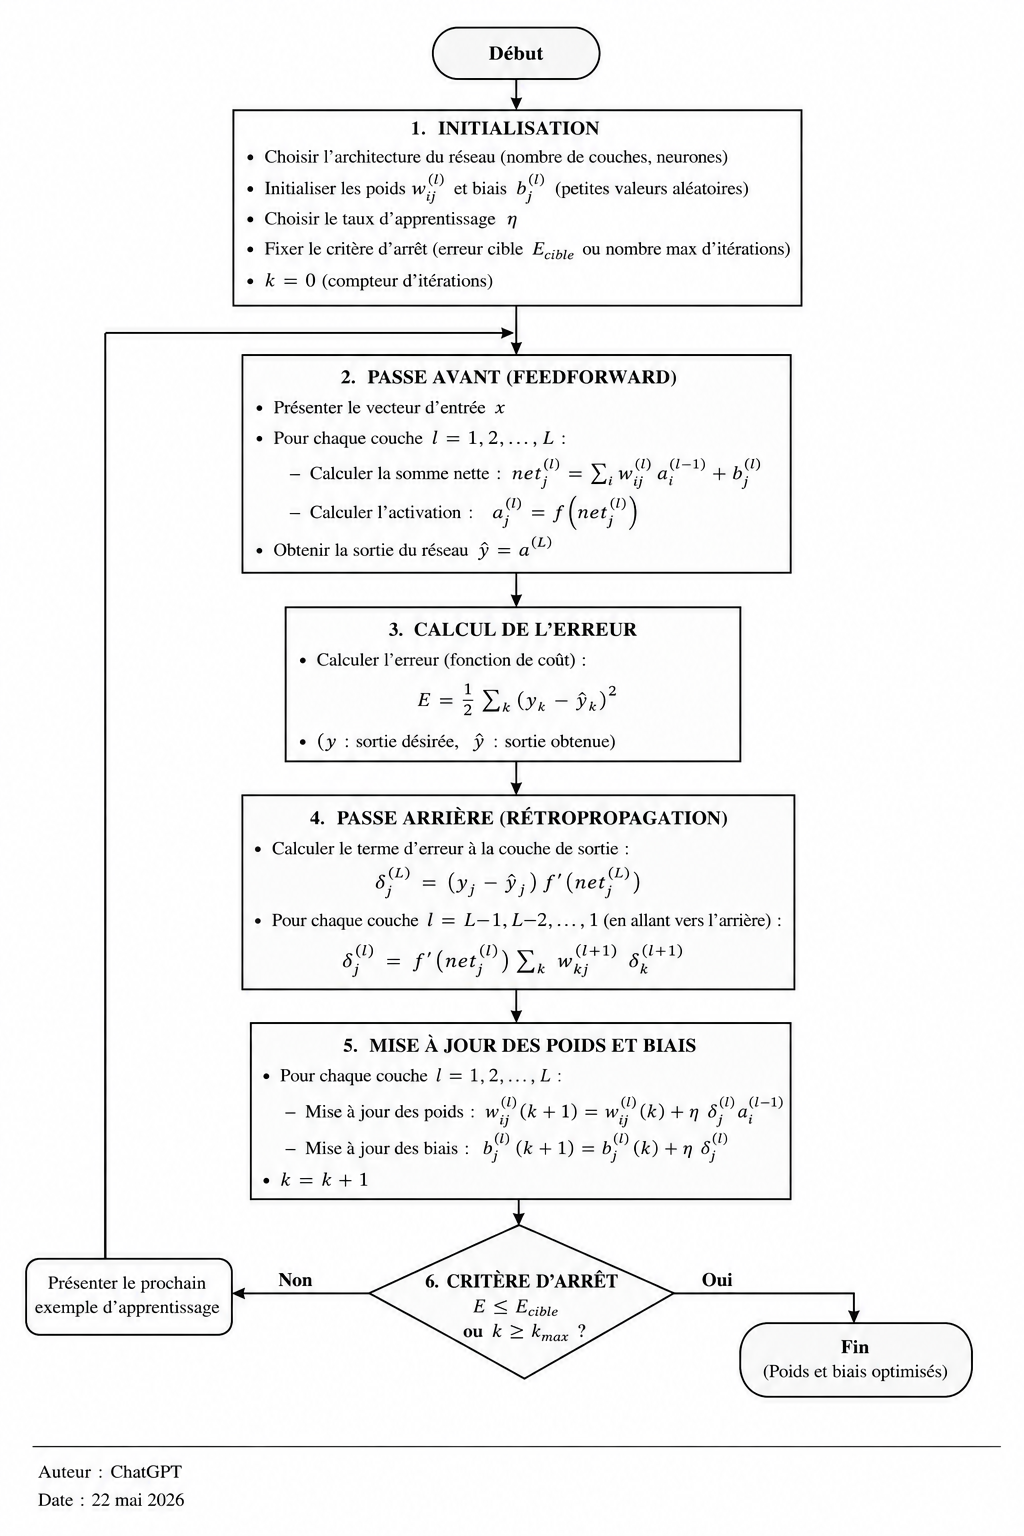
\includegraphics[width=0.8\textwidth]{./images/retropropagation}
	\caption{Organigramme de la rétro-propagation}
	\label{fig: retroprop}
\end{figure}

A la place de la fonction échelon comme fonction d'activation on peut utiliser la fonction $ReLU$, la fonction sigmoïde ou la fonction tangente hyperbolique. Comme vous pouvez le lire sur le site officiel de keras, il existe un grand nombre de fonction d'activation spécifiques à différentes tâches ou problèmes de \ac{ML}.

\subsection{Keras et Tensorflow}
Pour plus d'informations à propos de ces deux bibliothèques de python vous pouvez consulter les sites suivants : \url{https://www.tensorflow.org} et \url{https://keras.io}

\textbf{Keras} est une bibliothèque de haut niveau pour le deep learning, basée sur \textbf{Theano} et \textbf{TensorFlow}. Comme \ac{API} de haut niveau de TensorFlow, elle permet de créer et d'entraîner des modèles de deep learning. Elle est utilisé dans le cadre du prototypage rapide, de la recherche de pointe et du passage en production. Keras dispose d'une interface simple et cohérente, optimisée pour les cas d'utilisation courants ; ses modèles sont créés en connectant des composants configurables, avec quelques restrictions.

Quant à \textbf{TensorFlow}, c'est un outil open source d'apprentissage automatique développé par Google. Il prend en charge le deep learning, les réseaux de neurones et les calculs numériques généraux sur des \ac{CPU} et des \ac{GPU}. Il combine plusieurs modèles et algorithmes de \ac{ML} et les rend exploitables par le biais d'une interface commune.

Il existe trois façons de créer des modèles Keras:
\begin{itemize}
	\item \textbf{Le modèle séquentiel}, qui est très simple car c'est une liste de couches, mais qui se limite aux piles de couches à entrée unique et sortie unique.
	
	\item \textbf{L'\ac{API} fonctionnelle} est une \ac{API} complète et facile à utiliser qui prend en charge toutes les architectures de modèles.
	
	\item \textbf{Le sous-classement de modèles} consiste à tout implémenter soi-même.
\end{itemize}

Quant à l'entraînement du modèle, on fait appel à la méthode \textbf{fit} de l'objet \textbf{Sequential} ou \textbf{Model} instancié.

La méthode standard pour sauvegarder un modèle consiste à enregistrer l'intégralité du modèle dans un seul fichier avec \textbf{model.save()}. Le chargement du modèle sauvegardé se fait par la fonction \textbf{keras.models.load\_model}

\begin{lstlisting}
	# sauvegarde
	model=...
	model.save("path/to/location.keras")
	
	# chargement
	model = keras.models.load_model("path/to/location.keras")
\end{lstlisting}

Le fichier de sauvegarde comprend l'architecture du modèle, les valeurs des poids du modèle, la configuration d'entraînement du modèle...

\subsection{Construction d'un réseau de neurones avec l'API Sequential de Keras}

Un modèle séquentiel convient à une simple pile de couches où chaque couche possède exactement un tenseur d'entrée et un tenseur de sortie. Un tel modèle n'est pas approprié lorsque le modèle possède plusieurs entrées ou plusieurs sorties ; lorsque chaque couche possède plusieurs entrées ou plusieurs sorties ; ou lorsque nous avons besoin d'une topologie non linéaire.

Pour créer un modèle séquentiel, on peut soit passer une liste de couches au constructeur séquentiel, couches qui seront accessibles via l'attribut \textbf{layers} de la classe \textbf{keras.Sequential}; soit de manière incrémentale via la méthode \textbf{add} de cette classe. Pour supprimer les couches, on utilise la méthode \textbf{pop}.

\begin{lstlisting}
	from tensorflow import keras
	
	model = keras.Sequential()
	model.add(keras.layers.Dense(2,activation="relu", name="couche1"))
	model.add(keras.layers.Dense(3, activation="relu", name="couche2"))
	model.add(keras.layers.Dense(4, name="couche3"))
\end{lstlisting}

Pour permettre au modèle de connaitre la forme de son entrée et donc de déterminer la forme de la sortie, il faut l'initialiser en lui passant l'objet \textbf{Input}.
Une fois le modèle construit, on appelle sa méthode \textbf{summary} pour afficher son contenu ou son état.

\begin{lstlisting}
	model = keras.Sequential()
	model.add(keras.Input(shape=(4,)))
	model.add(layers.Dense(2, activation="relu"))
	model.summary()
\end{lstlisting}

Une fois l'élaboration du modèle terminée, on passe à l'entraînement. Cette phase consiste à entrainer le modèle, le valider sur un jeu de validation et de l'évaluer sur les données de test.

Premièrement, on spécifie la configuration d'entraînement avec la méthode \textbf{compile} où nous indiquons l'optimiseur, la fonction de coût et  les métriques. Si le modèle possède plusieurs sorties, on peut spécifier des fonctions de perte et des métriques différentes pour chaque sortie, et moduler la contribution de chacune à la perte totale du modèle. Ensuite, on appelle la méthode \textbf{fit} en lui fournissant comme paramètres les données d'entraînement, le nombre de lots(\textbf{batch\_size}) et le nombre d'époques.

On peut instancier l'optimiseur comme un objet du paquet \textbf{keras.optimizers} avant de le transmettre à la compilation ou le transmettre par son identifiant comme chaîne de caractères(les paramètres par défaut de l'optimiseur sont alors utilisés). Il est possible d'utiliser un programme de taux d'apprentissage pour contrôler la façon dont le taux d'apprentissage de l'optimiseur évolue dans le temps.

\begin{lstlisting}
	# Exemple d'une plannification
	lr_plan = keras.optimizers.schedules.ExponentialDecay(
	    initial_learning_rate=1e-2,
		decay_steps=10000,
		decay_rate=0.9
	)
	
	model.compile(
		optimizer=keras.optimizers.RMSprop(learning_rate=lr_plan),
		loss=keras.losses.SparseCategoricalCrossentropy(),
		metrics=[keras.metrics.SparseCategoricalAccuracy()],
	)
	
	history = model.fit(
		x_train,
		y_train,
		batch_size=64,
		epochs=2,
		validation_data=(x_val, y_val),
	)
\end{lstlisting}

L'objet \textbf{history} renvoyé contient un enregistrement des valeurs de perte et des valeurs des métriques pendant l'entraînement sous forme d'un dictionnaire.
Parmi les plans de taux d'apprentissage que propose keras, nous pouvons citer : \textbf{ExponentialDecay, CosineDecay, PolynomialDecay et InverseTimeDecay}.


Pour évaluer le modèle sur les données de test, on utilise la méthode \textbf{evaluate}. La prédiction sur des nouvelles données se fait par la méthode \textbf{predict}.

\begin{lstlisting}
	resulats = model.evaluate(x_test, y_test, batch_size=128)
	print("test loss, test acc: ", resultats)
	
	predictions = model.predict(x_test[:3])
\end{lstlisting}

\subsection{Construction d'un réseau de neurones avec l'API fonctionnelle}
L'API fonctionnelle permet de créer des modèles plus flexibles que l'API séquentielle. Elle peut gérer des modèles à topologie non linéaire, des couches partagées, et même plusieurs entrées ou sorties.

Voyons son fonctionnement à travers ce petit exemple

\begin{lstlisting}
	inputs = keras.Input(shape=(500,))
	dense = keras.layers.Dense(64, activation="relu")
	x = dense(inputs)
	x = keras.layers.Dense(64, activation="relu")(x)
	outputs = layers.Dense(10)(x)
	
	model = keras.Model(inputs=inputs, outputs=outputs)
	model.summary()
	
	keras.utils.plot_model(model, "model.png", show_shapes=True)
\end{lstlisting}

la fonction \textbf{keras.utils.plot\_model} nous permet de visualiser le modèle sous forme de graphique, ce qui nous montre clairement que l'API fonctionnelle permet de construire des graphes de couches.

\subsection{Utilisation des rappels (Callbacks)}

\begin{defi}[\textbf{Rappel}]
	Un rappel est un objet qui peut effectuer des actions à différentes étapes de l'entraînement : au début ou à la fin d'une époque, avant ou après un lot unique, au début ou à la fin de l'entrainement.
\end{defi}

La méthode \texttt{fit()} accepte un argument \texttt{callbacks} permettant de spécifier la liste des rappels. Par exemple, afin d'enregistrer des points de reprise intermédiaires du modèle et d'interrompre l'entraînement lorsqu'il n'y a plus d'amélioration, on utilise respectivement les classes \texttt{ModelCheckpoint} et \texttt{EarlyStopping}(Arrêt Précoce). Un rappel peut aussi servir à obtenir un aperçu des états internes et des statistiques d'un modèle pendant l'entraînement. Keras propose plusieurs fonctions de rappel telles que \textbf{ModelCheckpoint}(pour sauvegarder le modèle ou ses poids à une certaine fréquence), \textbf{BackupAndRestore}(pour sauvegarder et restaurer l'état d'entrainement, permettant de reprendre l'entrainement interrompu durant l'exécution de la méthode \textbf{fit}), \textbf{LearningRateScheduler}(à chaque époque, il récupère le taux d'apprentissage mis à jour et l'applique à l'optimiseur). Pour créer une nouvelle fonction de rappel, on crée une classe fille de \textbf{keras.callbacks.Callback} et on remplace la méthode associé à l'étape qui nous intéresse.

\begin{lstlisting}
	checkpoint = tf.keras.callbacks.ModelCheckpoint(
	"my_model.keras", save_best_weights=True)
	history = model.fit(X_train, y_train, epochs=10, callbacks=[checkpoint])
\end{lstlisting}

Le rappel \texttt{EarlyStopping} interrompt l'entraînement lorsqu'il ne constate plus aucun progrès sur le jeu de validation, au bout d'un certain nombre d'époques (fixé dans l'argument \texttt{patience}), et il revient automatiquement au meilleur modèle à la fin de l'entraînement si vous mettez \texttt{restore\_best\_weights} à \textbf{True}.

\begin{lstlisting}
	early_stopping = tf.keras.callbacks.EarlyStopping(
	patience=10, restore_best_weights=True)
\end{lstlisting}

\begin{lstlisting}
	# Rappel personnalise
	
	training_finished = False
	class MyCallback(Callback):
		def on_train_end(self, logs=None):
			global training_finished
			training_finished = True
	
	model = ...
	model.compile(loss="mean_squared_error")
	model.fit(np.array([[1.0]]), np.array([[1.0]]), callbacks=[MyCallback()])
\end{lstlisting}

\subsection{Réseaux de neurones convolutifs}
Considérons une image de $1000 \times 1000$ pixels en niveau de gris que nous souhaitons utilisée pour entrainer un modèle de reconnaissance d'image. Une telle image représente $10^6$ valeurs. Connecter chaque pixel à plusieurs neurones nous conduit à un nombre de connexions énormes, qui augmente donc la taille du modèle. Malheureusement, c'est la taille du modèle que nous devons optimiser car nos ressources sont très limitées!

Aussi, utiliser un perceptron multicouche sur de telles données n'est pas non plus efficace étant donné que les réseaux denses perdent l'organisation spatiale de l'image. D'où la nécessité de basculer vers des \textbf{réseaux convolutifs}.

\begin{defi}[Réseau de neurones convolutif]
	Un \ac{CNN} est un réseau de neurones spécialement conçu pour exploiter la structure locale des données. Il utilise des \textbf{filtres} qui se déplacent sur l'image pour produire des \textbf{cartes de caractéristiques} ou \textbf{feature maps}.
\end{defi}

Un \ac{CNN} commence par détecter des formes simples comme des bords, ensuite les formes et motifs complexes. Ceci est rendu possible grâce aux filtres et à la convolution. Un filtre n'est qu'une matrice(dans le cas d'une image à un canal comme dans notre cas) dont les coefficients sont appelés \textbf{poids du filtre}.

\begin{defi}[Convolution]
	Une convolution consiste à faire passer un petit filtre sur différentes régions de l'image, et à chaque région calculer la somme des produits des coefficients de même indices.
\end{defi}

Le \ac{CNN} apprend lui-même les poids des filtres durant l'entrainement. Ce sont des paramètres optimisés pendant l'apprentissage.

\begin{defi}[feature maps]
	Lorsqu'on applique un filtre à une image, on obtient une nouvelle matrice que l'on appelle feature map ou carte de caractéristiques. Chaque filtre génère sa propre carte, ce qui permet d'apprendre à détecter de caractéristique différente.
\end{defi}

\begin{figure}[H]
	% From ChatGpt
	\centering
	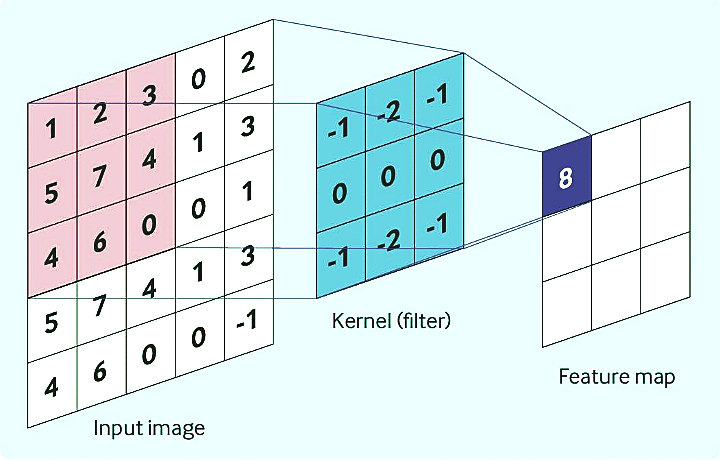
\includegraphics[width=0.7\textwidth]{./images/convolution}
	\caption{La convolution}
	\label{fig:convolution}
\end{figure}

Le pas de déplacement ou \textbf{stride} indique de combien de pixels le filtre se déplace. Plus sa valeur augmente, plus la sortie spatiale diminue. En plus, pour une image $5 \times 5$ et un filtre $3 \times 3$ avec un pas de 1, la carte de caractéristiques sera de taille $3 \times 3$ ; pour éviter cette réduction de taille, on ajoute des 0 au bords du feature map. C'est le \textbf{padding}.

Après certaines convolutions, on réduit généralement la taille des features maps afin de réduire la quantité de données, le coût des calculs et conserver les caractéristiques importantes. Pour ce faire, on utilise l'opération dite \textbf{Max Pooling} qui pour une matrice de taille donnée, retourne le coefficient maximal.

Voici une architecture typique d'un \ac{CNN} : une couche de convolution, suivi de la fonction d'activation, suivi d'une couche de \textbf{pooling}, suivi d'une autre couche de convolution, d'une fonction d'activation et d'une couche de \textbf{pooling}. Ensuite vient la couche d'aplatissement(\textbf{Flatten}), une couche dense et la classification.

\begin{figure}[H]
	\centering
	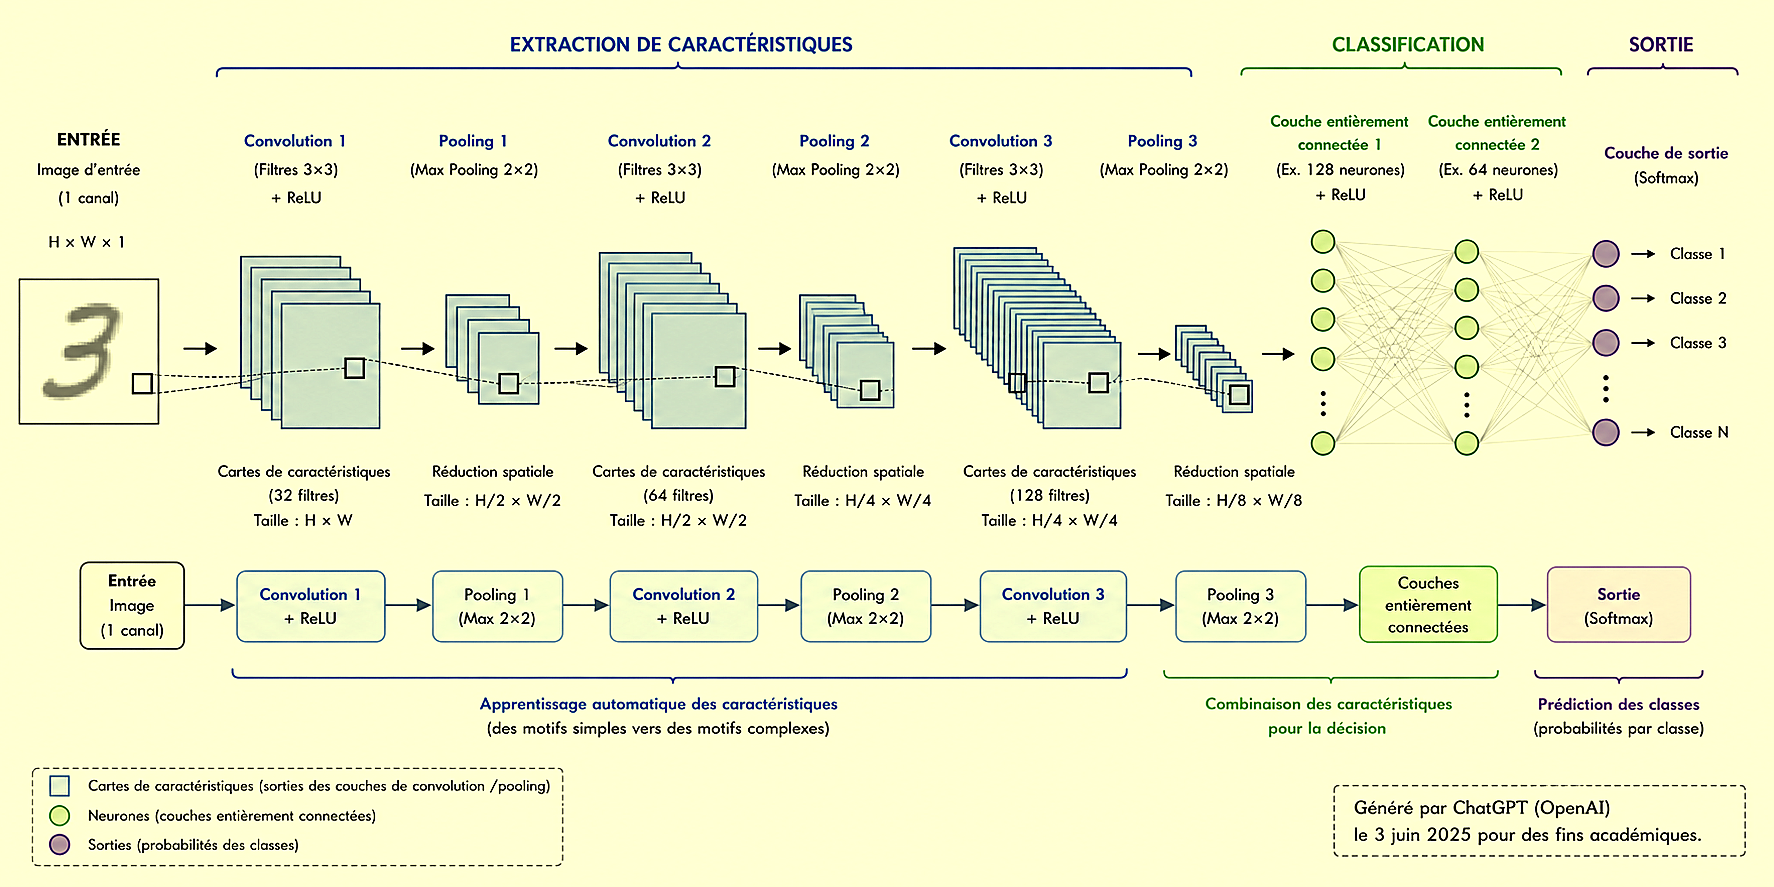
\includegraphics[width=1\textwidth]{./images/cnn}
	\caption{Architecture typique d'un \ac{CNN}}
	\label{fig:archi-cnn}
\end{figure}

Les \ac{CNN} sont efficaces dans l'analyse des images pour des raisons suivantes~:
\begin{itemize}
	\item Chaque filtre se focalise sur une petite région et l'étudie en particulier;
	\item Le même filtre est utilisé à plusieurs endroits(le partage des poids entre filtres) ce qui réduit le nombre des paramètres à entrainer;
	\item On peut réaliser une réduction de la taille des données à analyser pour optimiser la taille du modèle.
\end{itemize}

Dans le cas particulier de notre modèle de classification à 6 classes : \textbf{go, up, down, stop, left, inconnu}, devons reconnaitre des signaux vocaux en les classant comme membres de nos 6 régions de décision. Une commande vocale brute peut être représentée par des milliers d'échantillons ; faire fonctionner le réseau sur ces échantillons est coûteux. Afin de contourner ce problème, nous optons pour un changement de représentation, passer d'une liste d'échantillon à une représentation plus compacte basée sur les caractéristiques fréquentielles importantes.

Cette nouvelle représentation ressemble conceptuellement à une image. Nous pourrons donc implémenter un \ac{CNN} pour traiter notre problème. 

\section{Spectrogramme Mel}
\begin{defi}[Spectrogramme Mel]
	Le spectrogramme en échelle Mel est une représentation visuelle d'un signal audio qui montre comment son énergie fréquentielle évolue dans le temps, adapté à la façon dont l'oreille humaine perçoit les sons.
\end{defi}

Il répond à deux questions~:
\begin{itemize}
	\item transformer le son en une image en deux dimensions(temps, fréquence).
	\item réduire cette image à une taille compatible avec les ressources très limitées d'un micro-contrôleur, tout en conservant l'information pertinente.
\end{itemize}

Un son numérique est une suite d'échantillons prélevés à une fréquence d'échantillonnage donnée($\SI{16000}{\hertz}$ dans notre cas). Comme le contenu fréquentiel de la parole change beaucoup, on ne calcule pas le spectre sur tout le clip audio d'un seul coup, on découpe le signal en petites \textbf{fenêtres} qui se chevauchent légèrement.

Dans ce projet, chaque fenêtre couvre $30ms$(soit $480$ échantillons à $\SI{16}{\kilo\hertz}$), et on avance de $20ms$(soit $320$ échantillons) entre deux fenêtres consécutives. Ce chevauchement de $10ms$ évite de perdre de l'information aux bords de chaque fenêtre.

Avant de calculer la transformée de Fourier, on multiplie chaque fenêtre par une \textbf{fenêtre de Hamming}, qui atténue les bords du segment~:
\[w[n] = 0.54 - 0.46\cos(\frac{2\pi n}{N-1}), \large n=0,...,N-1\]
La \textbf{transformée de Fourier discrète} décompose un signal temporel en une somme de sinusoïdes de fréquences différentes.

\begin{defi}[\ac{FFT}]
    La transformée de Fourier rapide est un algorithme qui calcule la transformée de Fourier discrète en \textbf{$O(N\log N)$} opérations au lieu de \textbf{$0(N^2)$}, le rendant très pratique pour un microcontrôleur.
\end{defi}

Pour une fenêtre de $N=512$ points, la \ac{FFT} produit un spectre complexe de $\frac{N}{2} + 1=257$ fréquences distinctes représentables. Le spectre contient donc $257$ valeurs réparties linéairement.

Afin de résoudre des problèmes de perception et de taille de données à fournir au modèle que l'échelle Mel(construite expérimentalement en 1937) est introduite. La relation entre la fréquence physique et la hauteur perçue n'est pas linéaire mais approximativement logarithmique au delà de $\SI{1000}{\hertz}$.

La formulation la plus répandue de l'échelle Mel est la \textbf{formule de Slaney}, qui donne le nombre de mels m en fonction de la fréquence f~:
\[m(f) = 2595 \log(1 + \frac{f}{700})\]

\subsection{Construction du banc de filtres Mel}
Le banc de filtre Mel transforme le spectre de puissance linéaire en un petit nombre de bandes d'énergie(40 dans le projet), réparties selon l'échelle Mel. Chaque filtre m est une fonction triangulaire qui vaut 0 en dehors de sa plage de fréquences, monte linéairement jusqu'à 1 en son centre, puis redescent linéairement jusqu'à 0. Pour chaque filtre m, l'énergie mel correspondante s'obtient en sommant le spectre de puissance pondéré par les poids du filtre.
\subsection{Pourquoi précalculer les filtres en Python}
Les poids des filtres ne dépendent que des paramètres choisis une fois pour toutes(la fréquence d'échantillonnage, le nombre d'échantillons d'une fenêtre, le nombre de filtres, la fréquence maximale et la fréquence minimale) et non du son capté en temps réel. Le script \textbf{export\_mel\_filterbank.py} que vous trouverez sur github, utilise \textbf{librosa.filters.mel()} pour calculer cette matrice une seule fois, puis génère un fichier d'en-tête C contenant les poids. Le microcontrôleur n'a alors plus qu'à faire des multiplications-additions à chaque trame.

\section{Mise au point de notre modèle de classification multiclasse}

Ce modèle est inspiré de ceux proposés par les développeurs de tensorflow lors de la réalisation de l'exemple \textbf{micro-speech}. Leurs codes sont disponibles sur Github(\url{https://github.com/tensorflow/tensorflow.git}). 

\begin{lstlisting}
	from tensorflow import keras
	# Inspiree du code speech_commands/models.py
	# du depot https://github.com/tensorflow/tensorflow.git
	
	def model_convolution(input_shape=(49, 40, 1), nbre_classes: int = 6):
		inputs = keras.Input(shape=input_shape)
		conv1 = keras.layers.Conv2D(
			filters=16,
			kernel_size=(10, 8),
			strides=(2, 2),
			padding="same",
			use_bias=False,
			activation="relu",
			name="conv_1"
		) # Premiere couche de convolution
		bn1 = keras.layers.BatchNormalization(name="BNormalisation1")
		pooling1 = keras.layers.MaxPooling2D()
		
		conv2 = keras.layers.Conv2D(
			filters=32,
			kernel_size=(10, 8),
			strides=(2, 2),
			padding="same",
			use_bias=False,
			activation="relu",
			name="conv_2"
		) # Deuxieme couche de convolution
		
		bn2 = keras.layers.BatchNormalization(name="BNormalisation2")
		pooling2 = keras.layers.MaxPooling2D()
		dropout1 = keras.layers.Dropout(0.3, name="dropout_1") # Couche de regularisation
		
		global_pool = keras.layers.GlobalAveragePooling2D()
		
		dense_hidden = keras.layers.Dense(
			32,
			activation="relu",
			kernel_regularizer=keras.regularizers.l2(1e-4),
			name="couche_cachee"
		)
		
		dropout2 = keras.layers.Dropout(0.3, name="dropout_2")
		
		couche_sortie = keras.layers.Dense(
			nbre_classes,
			activation="softmax",
			kernel_regularizer=keras.regularizers.l2(1e-4),
			name="output_dense"
		)
		
		x = conv1(inputs)
		x = bn1(x)
		x = pooling1(x)
		
		x = conv2(x)
		x = bn2(x)
		x = pooling2(x)
		
		x = dropout1(x)
		x = global_pool(x)
		x = dense_hidden(x)
		x = dropout2(x)
		outputs = couche_sortie(x)
		
		model = keras.Model(
			inputs=inputs,
			outputs=outputs,
			name="Tiny_Embedding_Conv_Audio"
		)
		
		return model
\end{lstlisting}
 
 Le résumé ci-dessous liste les informations relatives aux paramètres du modèle ainsi que leurs contributions à la taille finale du modèle non quantifié. Cette taille est excellente car elle est déjà bien en dessous des limites mémoires de notre microcontrôleur avant même la quantification. Au total, $43686$ paramètres d'entrainement dont $96$ paramètres non entraînables, pour une taille totale de \SI{170.65}{\kilo\byte}.
 
 \begin{figure}[H]
 	\centering
 	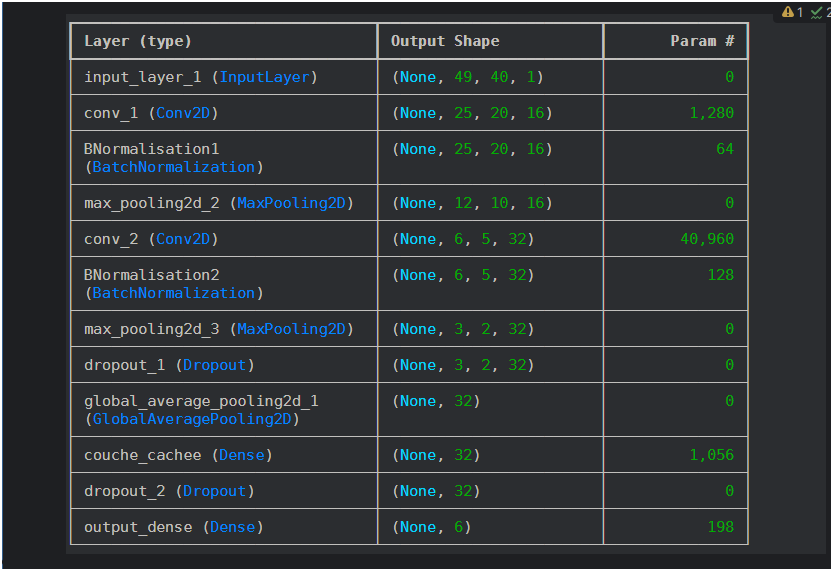
\includegraphics[width=0.7\textwidth]{images/resumeCNN}
 	\caption{Informations sur le modèle}
 	\label{fig:infocnn}
 \end{figure}
 
 Les courbes d'apprentissage de ce modèle nous indique un sur-apprentissage. Ceci est probablement dû à la quantité des données ou à la complexité du modèle, qui a alors du mal à généraliser. Cet écart est pourtant négligeable si nous tenons compte de notre objectif qui n'est que de commander un petit moteur ; pour des projets exigeants en terme de précision, il faut revoir les données et les hyperparamètres(en choisissant les plus adaptés). Notons aussi que nous n'avons pas tenu compte des bruits durant l'entrainement ce qui pourrait nuire au bon fonctionnement du modèle. La précision de ce modèle est autour de $90\%$, même pour la version \textbf{quantifiée} du modèle.
 
\begin{figure}[H]
	\centering
	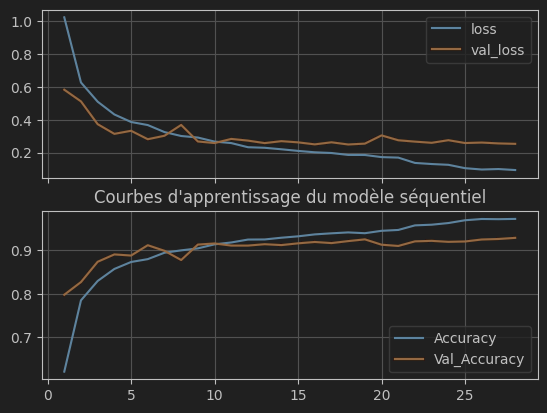
\includegraphics[width=0.7\linewidth]{images/courbes_apprentissage}
	\caption{Courbes d'apprentissage du modèle}
	\label{fig:courbesapprentissage}
\end{figure}

Par rapport aux données, nous avons utilisé le même dataset open-source que pour l'exemple micro-speech faute de données personnalisées. Le lien vers ce dataset est donné en annexe et le code d'extraction est disponible dans notre dépôt Github pour ce projet. La répartition des données est comme ci-dessous~:

\begin{verbatim}
	Données chargées : 23394
	go : 3880 échantillons
	up : 3723 échantillons
	down : 3917 échantillons
	left : 3801 échantillons
	stop : 3872 échantillons
	inconnu : 4201 échantillons
\end{verbatim}

$16375$ échantillons pour le jeu de données d'entrainement, $3509$ échantillons pour le jeu de données de validation et $3510$ échantillons pour le jeu de données de test. C'est à dire $15\%$ des données pour la validation, $15\%$ pour le test et $70\%$ des données pour l'entraînement. L'entrainement n'a duré que pendant \textbf{28 époques} grâce à un arrêt précoce. Ci-dessous est l'image de la matrice de confusion qui nous donne une idée claire sur la précision du modèle ; la diagonale représente les reconnaissances correctes et les cases hors diagonales indiquent quelle commande est confondue avec quelle autre.

\begin{figure}[H]
	\centering
	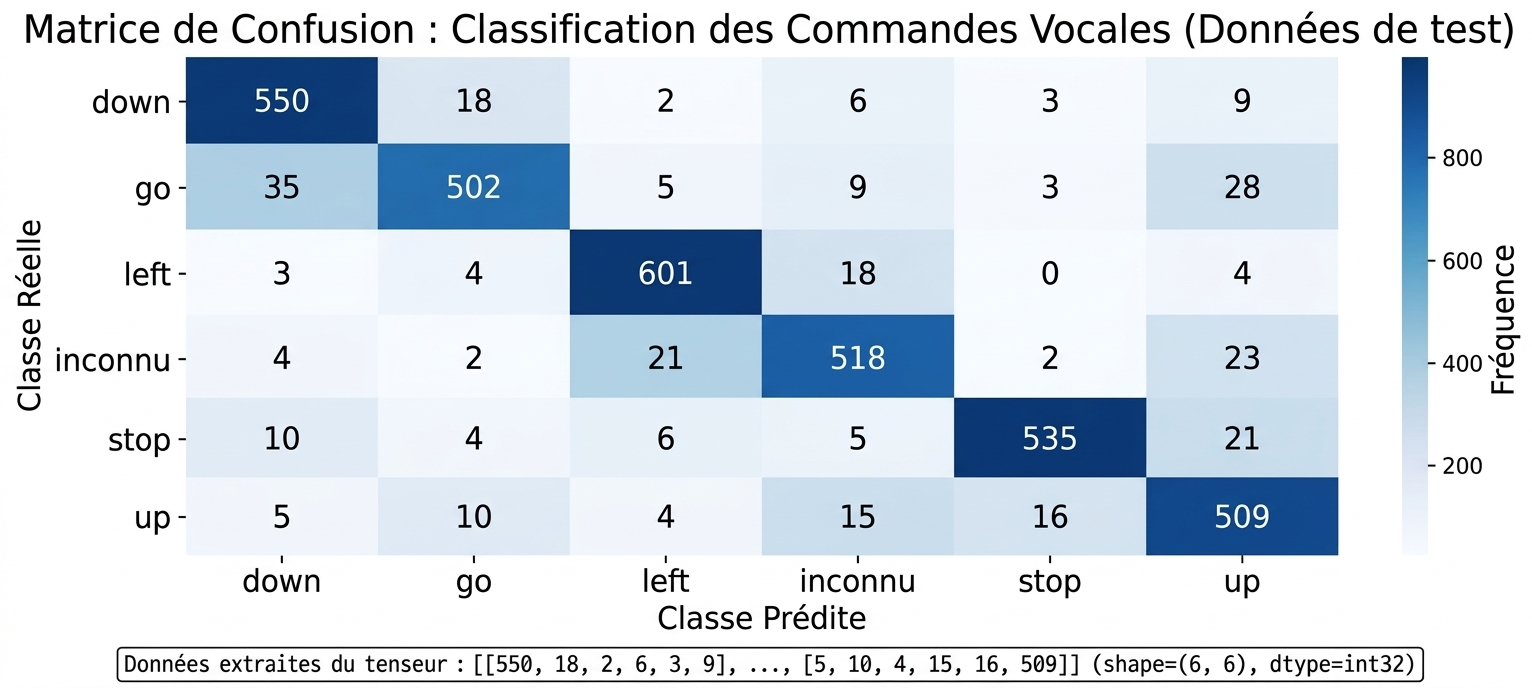
\includegraphics[width=0.9\textwidth]{images/matriceConfusion}
	\caption{Matrice de confusion du modèle}
	\label{fig:matriceconfu}
\end{figure}

\chapter{Analyse du moteur DC}

\section{Présentation du moteur}

\begin{figure}[H]
	\centering
	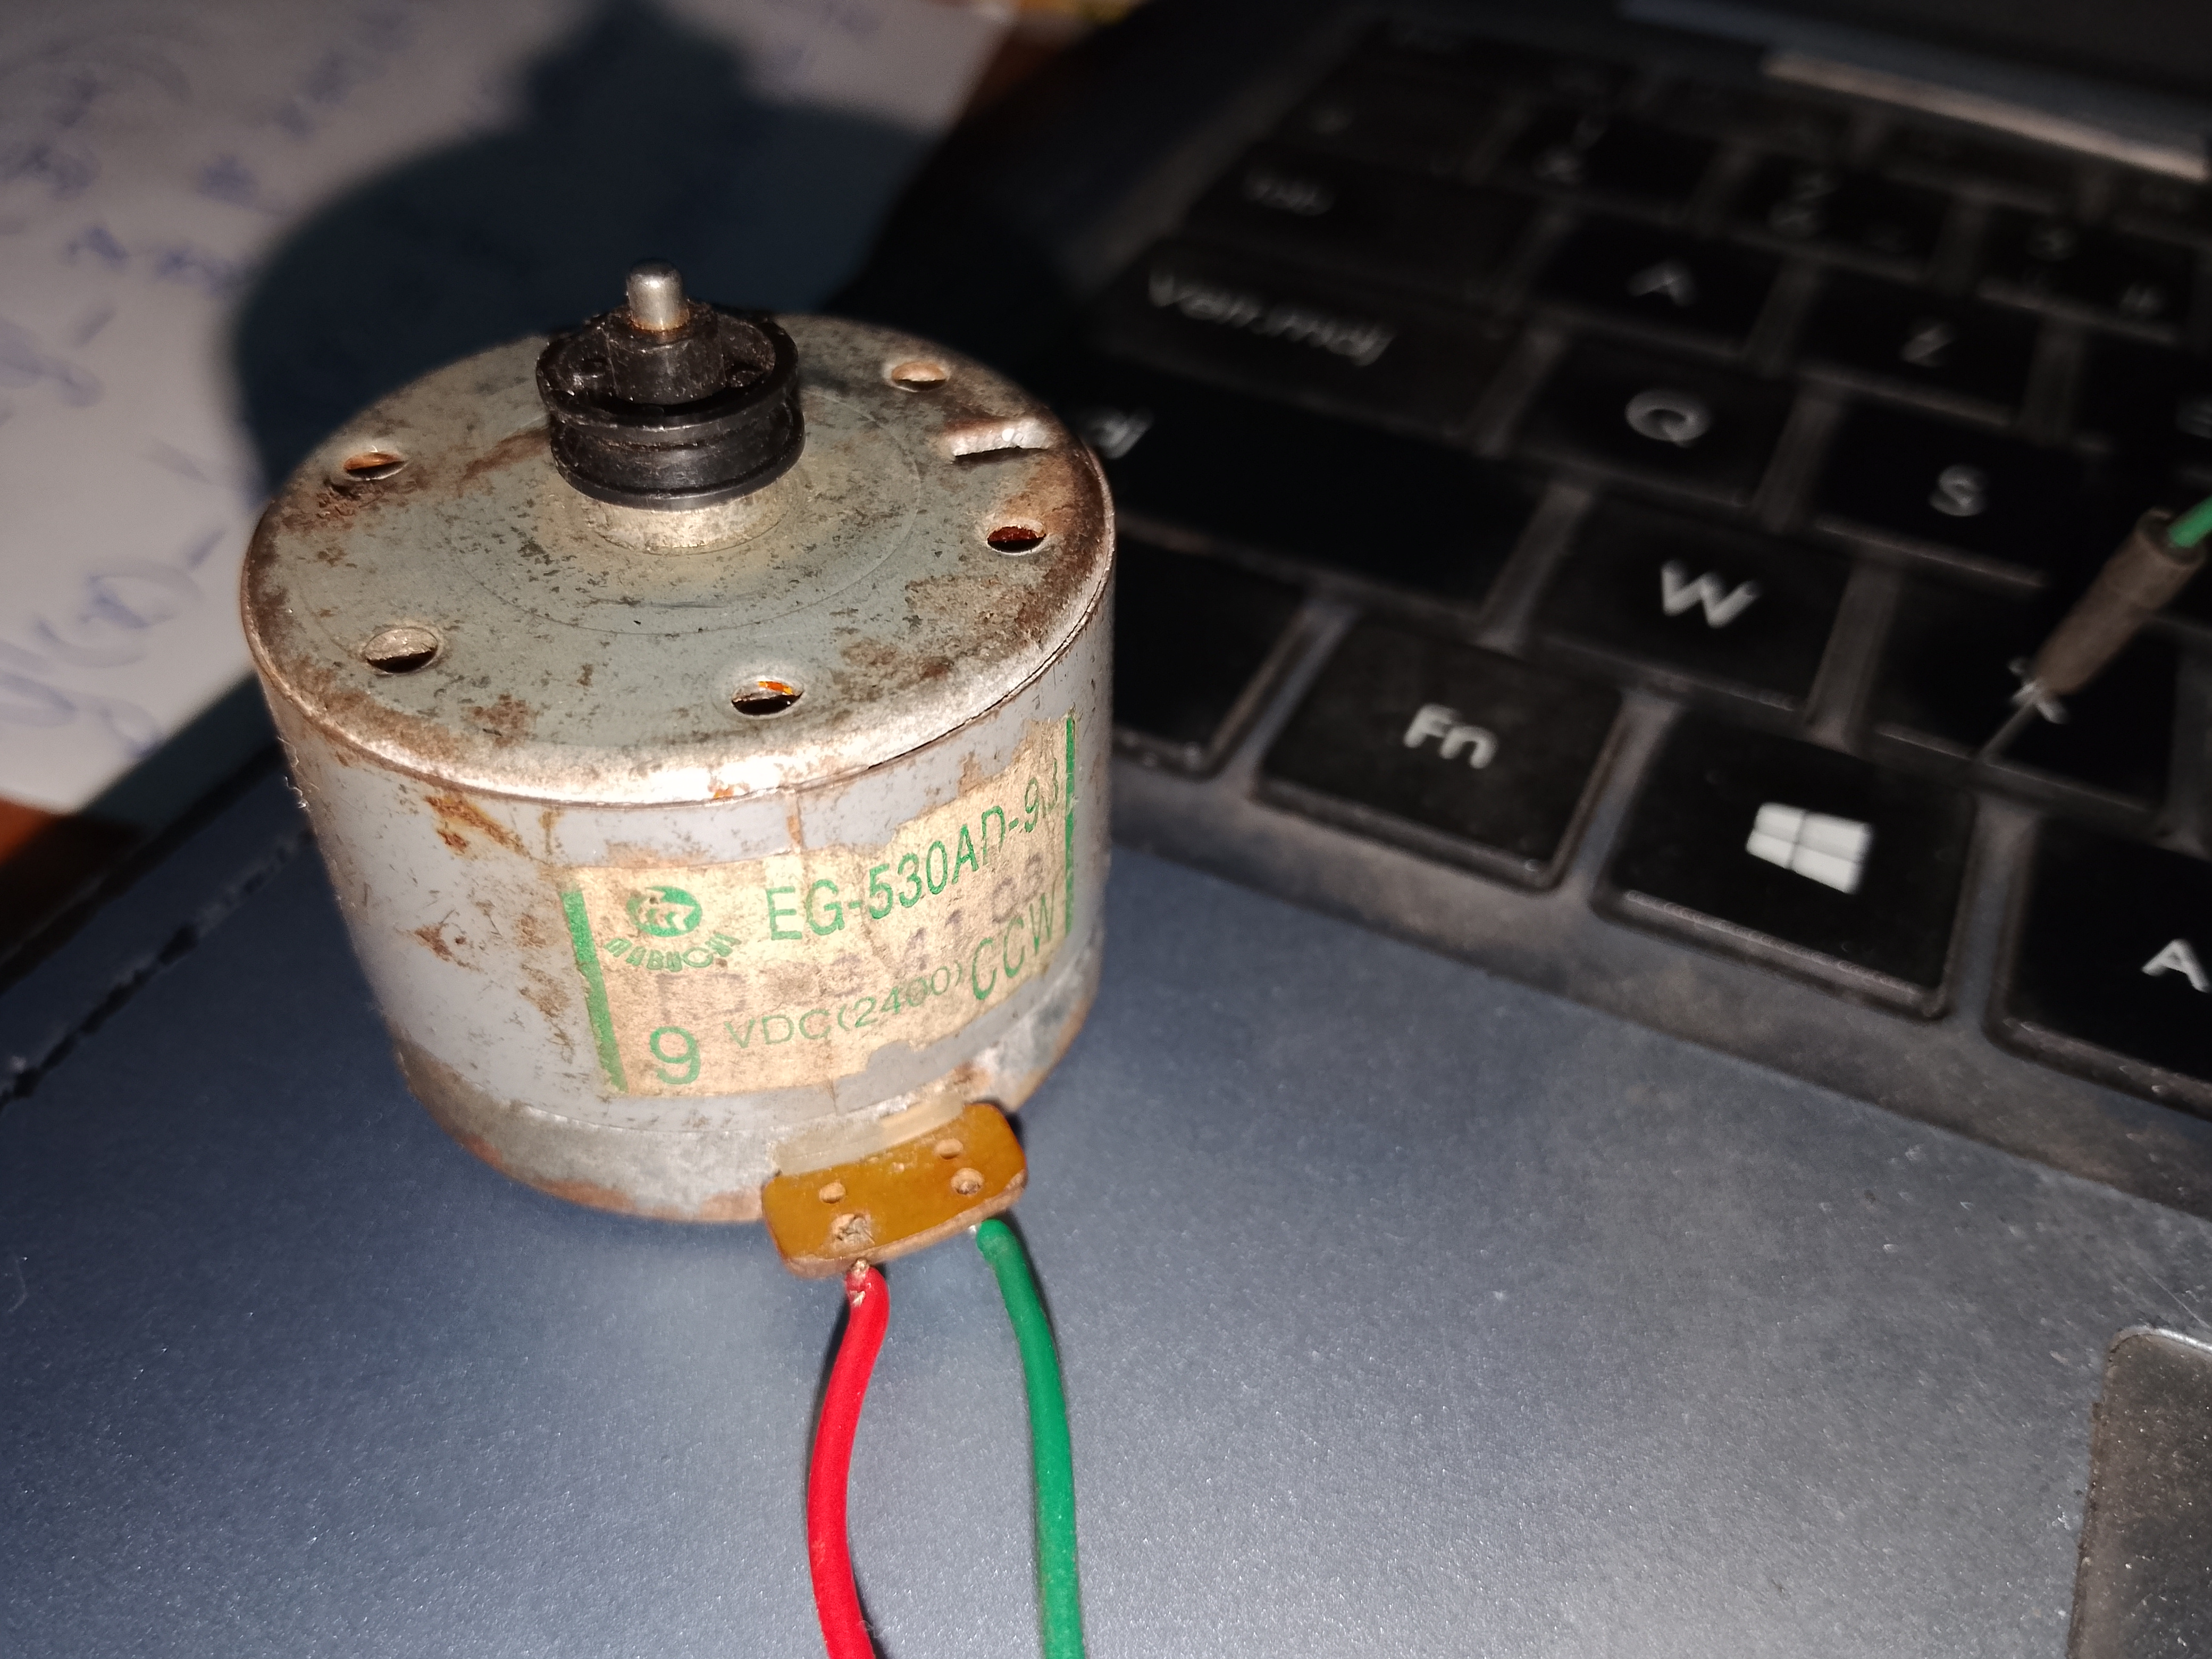
\includegraphics[width=0.6\textwidth]{./images/moteurDC}
	\caption{EG-530AD-9B}
	\label{fig:moteurDC}
\end{figure}

Nous utilisons un moteur à courant continu à aimant permanent de la série Mabuchi Motor EG-530AD, le EG-530AD-9B. C'est un petit moteur à balais qui équipait une ancienne radio cassette et dont nous avons relevé les caractéristiques électriques suivantes à partir de sa fiche technique\cite{moteur_datasheet}~:

\begin{itemize}
	\item tension nominale~: \SI{9}{\volt}~;
	\item plage de fonctionnement admissible en tension~: 6 à \SI{11}{\volt}~;
	\item couple nominal~: \SI{0.78}{\milli\newton\meter} (\SI{8}{\gram\centi\meter})~;
	\item vitesse nominale~: $2400 \pm 48\ \si{tr/min}$.
\end{itemize}

La fiche technique de ce moteur \ac{DC}, de \SI{70}{\gram}, fournit aussi les caractéristiques courant d'alimentation--couple pour trois valeurs de tension d'alimentation.

\begin{figure}[H]
	\centering
	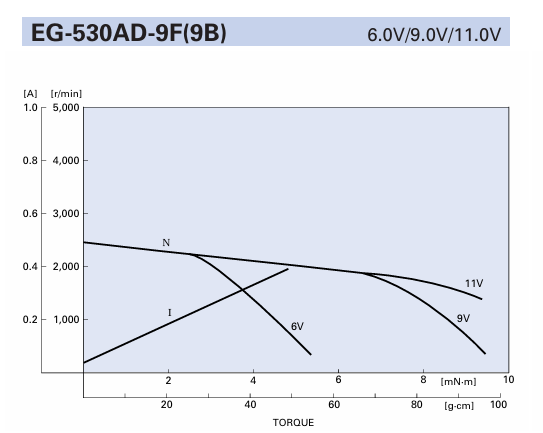
\includegraphics[width=0.7\textwidth]{./images/moteurCaracteristiques}
	\caption{Courbe $I_a = f(C)$ extraite de la fiche technique du moteur EG-530AD-9B}
	\label{fig:Ia_fC}
\end{figure}

Comme nous l'avons souligné au début, le moteur est ancien et connaît donc le vieillissement. Pour nous rassurer sur ses performances, nous avons réalisé deux essais au laboratoire d'électronique de la faculté~: l'essai à vide ainsi que l'essai à rotor bloqué, pour déterminer le courant maximal appelé par le moteur. Durant l'essai à vide, nous avons pris la peine de ne considérer que le courant de démarrage. Voici les résultats de ces essais que vous pouvez retrouver sur GitHub dans le dépôt \url{https://github.com/robohie/prog_python}, à l'intérieur du dossier \texttt{rapports/classeurs}.

\begin{figure}[H]
	\centering
	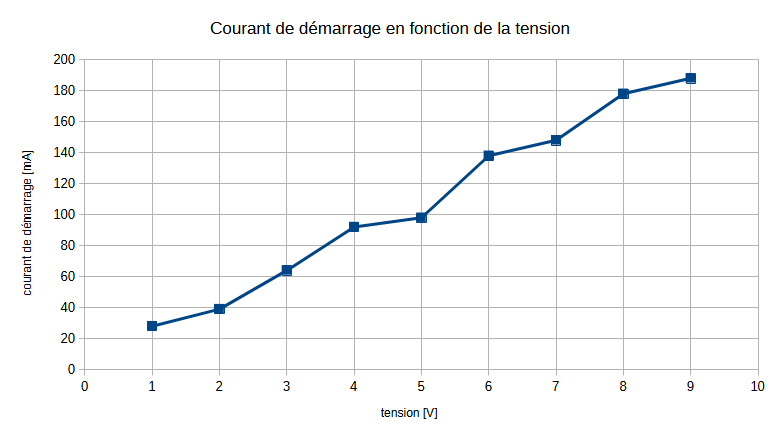
\includegraphics[width=0.8\textwidth]{./images/courantDemarrage}
	\caption{Essai à vide -- courant de démarrage}
	\label{fig:essai_vide}
\end{figure}

À \SI{9}{\volt}, avec le rotor bloqué, nous avons mesuré un courant de \SI{310}{\milli\ampere} avec un multimètre numérique. À $2400\ \si{tr/min}$ et \SI{9}{\volt}, nous avons mesuré un courant de démarrage maximal de \SI{193}{\milli\ampere}. Pour dimensionner les composants du circuit de commande du moteur, nous assumerons un facteur de sécurité de $2.5$ ; ainsi le courant de dimensionnement est \SI{775}{\milli\ampere}. Donc, les composants de commutation que nous allons utiliser doivent supporter un courant maximal supérieur à ce courant de dimensionnement, au moins \SI{1}{\ampere}.

\section{Modélisation du moteur pour la simulation}

\begin{figure}[H]
	\centering
	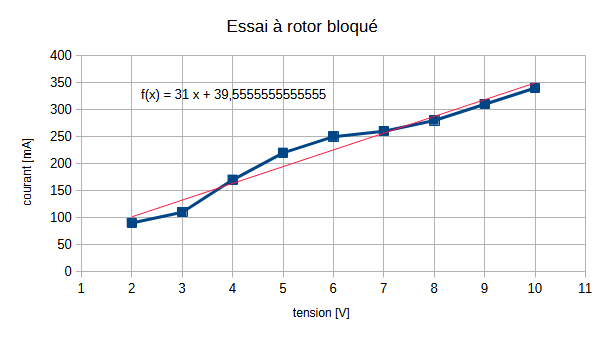
\includegraphics[width=0.8\textwidth]{./images/rotorBloque}
	\caption{Essai à rotor bloqué -- courant en fonction de la tension}
	\label{fig:essai_rotor_bloque}
\end{figure}

Afin de réaliser des simulations de notre moteur sur LTspice, nous le modélisons simplement comme la mise en série d'une résistance, d'une inductance et d'une source de tension (la force contre-électromotrice), sa résistance et son inductance étant déterminées par des mesures direct ou indirect.

\begin{figure}[H]
	\centering
	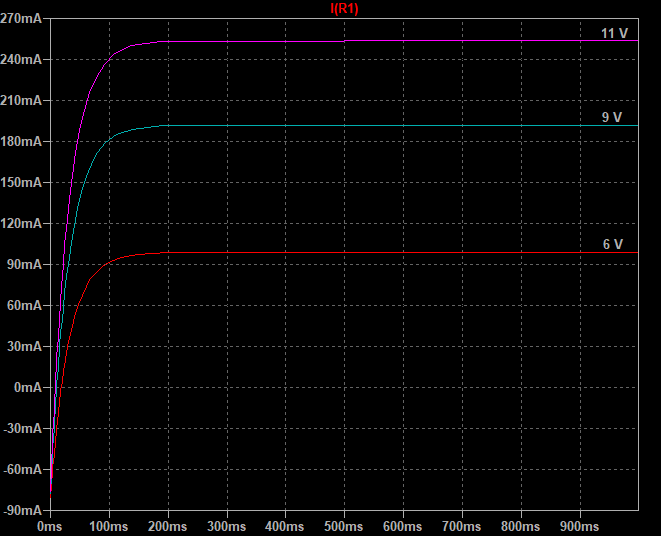
\includegraphics[width=0.7\linewidth]{images/model_moteurDC}
	\caption{Modèle du moteur sous LTspice}
	\label{fig:moteur_ltspice}
\end{figure}


À partir de l'essai à rotor bloqué, $V_a = R \cdot I_a$ avec $V_a = \SI{9}{\volt}$ et $I_a = \SI{310}{\milli\ampere}$. Le moteur a donc une résistance d'environ \SI{29}{\ohm}.
Afin de tenir compte des variations des données, nous avons déterminé la droite de régression linéaire à partir de \textbf{libreOffice Calc} ; ce classeur se trouve sur github, le lien est donné ci-dessus. L'équation de la droite est $i(V) = 31 \cdot V + 39.6~ [\SI{}{\milli\ampere}]$. La pente de cette équation représente la conductance en $\SI{}{\milli\siemens}$ ; en considérant son inverse nous avons la résistance du moteur : $\SI{32.3}{\ohm}$.

Appelons $E$ la force contre-électromotrice du moteur, et $R I_a$ la chute de tension aux bornes de la résistance interne du moteur. Le moteur étant à aimant permanent et tournant à une vitesse constante, la force contre-électromotrice est aussi constante suivant la relation $E = k\Phi\Omega$. $\Phi$ et le flux magnétique dans l'entrefer, $\Omega$ la vitesse angulaire.

Alors, la force contre-électromotrice est~:
\[ V_a = E + R I_a \quad \text{c.-à-d.} \quad E = V_a - R \cdot I_a \]
Pour $V_a = \SI{9}{\volt}$, $I_a = \SI{193}{\milli\ampere}$ (à $2400\ \si{tr/min}$), et $R = \SI{32.3}{\ohm}$, on obtient $E \simeq \SI{2.8}{\volt}$.

Quant à l'inductance de l'enroulement d'armature, nous considérons, par analogie avec d'autres moteurs à aimant permanent de mêmes dimensions, la valeur de $\SI{0.1}{\milli\henry}$.

\begin{figure}[H]
	\centering
	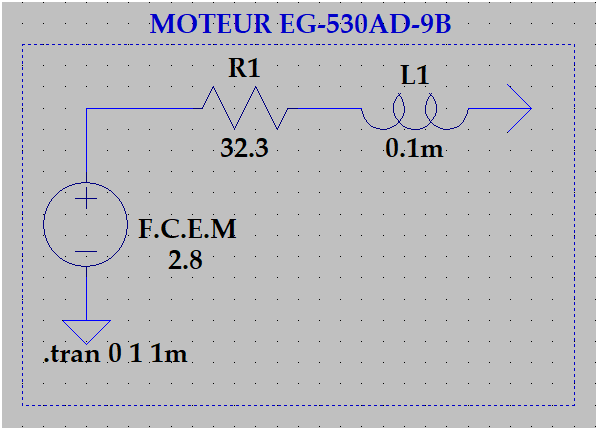
\includegraphics[width=0.7\linewidth]{images/schemaEquivalent}
	\caption{Schéma équivalent du moteur DC}
	\label{fig:schemaequivalent}
\end{figure}



\chapter{Conception du pont en H de commande du moteur}

\section{Les transistors}

\hfill\\
\emph{Références principales de cette section~: \cite{haas_mikulec_transistors,lamache_transistors}.}

Un transistor est un composant électronique possédant trois bornes qui permettent, grâce au courant ou  à la tension appliquée entre deux d'entre elles, de commander le courant à travers l'autre broche.

Nous distinguons deux grands types de transistor~: les transistors à effet de champ dont le \ac{JFET} et le \ac{MOSFET}, tels que la commande du courant qui circule au drain est assurée par la tension appliquée à la grille ; et le \ac{BJT} où un faible courant circulant à la base(un équivalent de la grille) contrôle les courants qui circulent au collecteur et à l'émetteur.

\subsubsection{Transistor à jonction bipolaire}

Un \ac{BJT} peut être de type NPN (la base est dopée P, entourée de deux régions dopées N, l'émetteur et collecteur) ou de type PNP (la base est dopée N, entourée de deux régions dopées P). Grâce à l'effet transistor, on trouve les relations suivantes entre le courant de base et le courant collecteur ainsi que le courant émetteur, dans la zone linéaire de fonctionnement du transistor($\beta$ est appelé gain)~:

\[ I_{\text{collecteur}} = \beta \cdot I_{\text{base}} \qquad I_{\text{émetteur}} = I_{\text{collecteur}} + I_{\text{base}} = (1 + \beta) I_{\text{base}} \]

\subsubsection{Transistors à effet de champ}
Par rapport aux \acp{BJT}, les \acp{MOSFET} consomment moins de puissance. Un \ac{MOSFET} est aussi un composant à trois broches(la grille, le drain et la source) telles que le courant du drain est contrôlé par une petite tension au niveau de la grille. Deux technologies de ce composant sont disponibles : le \ac{MOSFET} à enrichissement et le \ac{MOSFET} à appauvrissement. En appauvrissement, quand la tension de grille est faible ou nulle, le canal semiconducteur aura sa plus grande conductivité(il sera passant) ; en enrichissement, quand la tension de grille est faible ou nulle, le transistor est bloqué, pour augmenter la conductivité, une plus grande tension doit être appliquée.

Pour un \ac{MOSFET} donné, nous distinguons les grandeurs suivantes nécessaires au dimensionnement : la tension grille--source($V_{GS}$), la tension de seuil($V_{GS(seuil)}$), la tension drain--source($V_{DS}$), la résistance drain-source à l'état passant($R_{DS(on)}$) ainsi que la charge électrique totale($Q_g$) du condensateur d'entrée afin de tenir compte de la commutation.

On dit qu'un \ac{MOSFET} se trouve dans la zone ohmique ou linéaire, quand sa caractéristique de sortie $I_D = f(V_{DS})$ est linéaire. Ce mode correspond au mode de fonctionnement privilégié pour le faire fonctionner comme interrupteur. Par contre, il est dit en \textbf{saturation} quand son courant de drain est quasi invariant quelle que soit la tension $V_{DS}$. Dans ce mode, il fonctionne comme une source de courant.

\section{Le pont en H}

Le pont en H est un montage de quatre transistors permettant de connecter le  moteur \ac{DC} à son alimentation de diverses façons~\cite{epfl_moteurs_ponth_pwm,bichet_pwm_ponth}.

\begin{figure}[H]
	\centering
	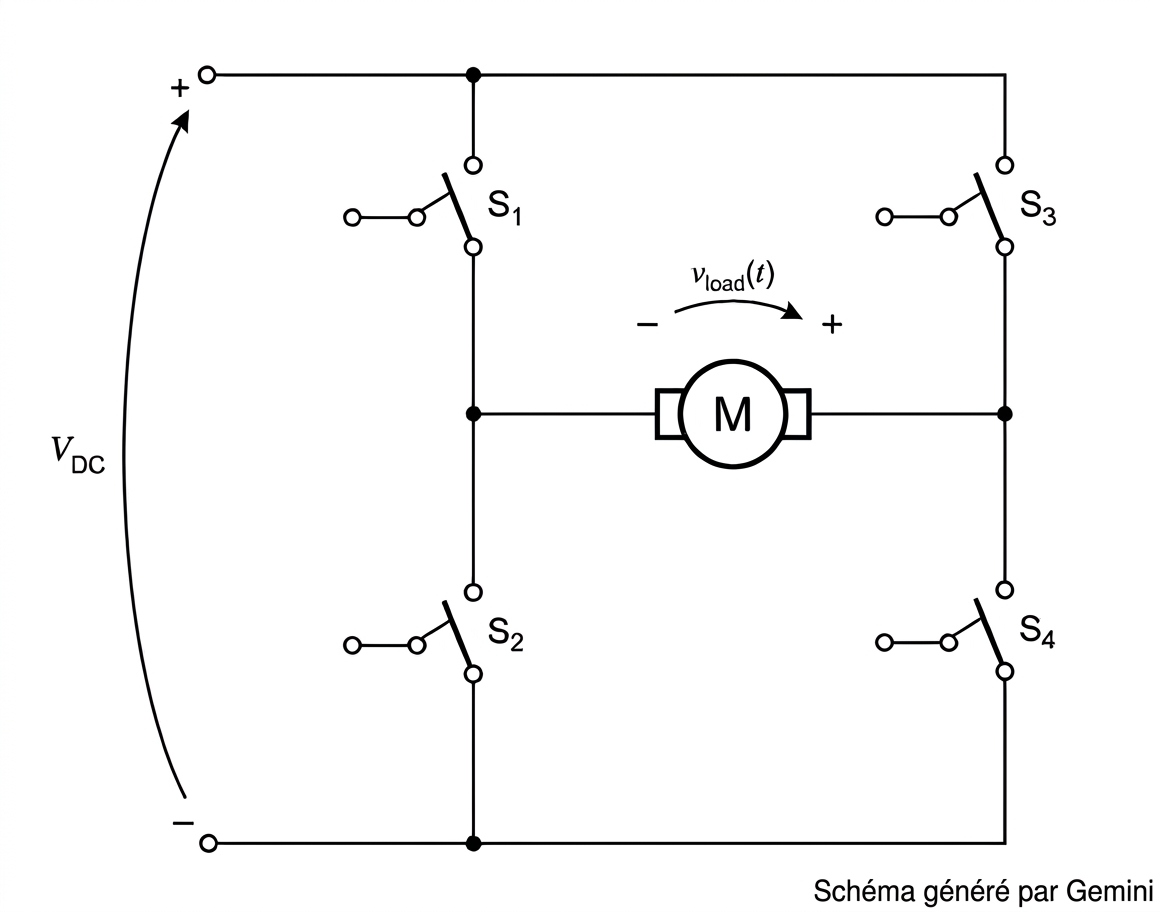
\includegraphics[width=0.6\textwidth]{images/principe_pontH}
	\caption{Schéma de principe du pont en H}
	\label{fig:pont_h}
\end{figure}

Par rapport à la figure ci-dessus~:
\begin{itemize}
	\item en fermant les interrupteurs 1 et 4, le courant passe à travers le moteur dans un sens~;
	\item en fermant les interrupteurs 2 et 3, le courant passe à travers le moteur dans l'autre sens;
	\item  en fermant les interrupteurs 1 et 2, nous provoquons un court-circuit, très dangereux pour les composants qui risquent alors de griller;
	\item de même fermer simultanément les interrupteurs 3 et 4, nous provoquons aussi un court-circuit;
	\item fermer les interrupteurs 1 et 3 (ou 2 et 4) met le moteur en freinage dynamique.
\end{itemize}

Comme la vitesse du moteur est fonction de la tension d'alimentation, et que nous souhaitons trouver un moyen de la modifier à volonté, nous devons recourir à une méthode permettant de varier la tension aux bornes du moteur. Pour ce faire, nous nous servons des broches PWM (Pulse Width Modulation) de l'Arduino Nano 33 \ac{BLE} Sense Rev2.

\subsection{La modulation de largeur d'impulsion (\ac{PWM})}

La modulation de largeur d'impulsion (\ac{PWM}) est une méthode permettant de générer des signaux analogiques à l'aide des systèmes en fonctionnement tout ou rien. Deux informations sont importantes à savoir, la période $T$ du signal carré et le rapport cyclique $d$. Ce dernier est le rapport du temps durant lequel le système est à l'état \textbf{haut} et la période i.e. $d=\frac{t_{on}}{T}$. Avec notre micro-contrôleur, nous pouvons générer un tel signal à partir des broches D2, D3, \ldots, D12 ou D13 par la fonction « analogWrite ». Le \ac{PWM} peut varier entre 0 et 255~; par exemple, pour $PWM= 127$, nous obtenons un signal carré d'amplitude moyenne correspondant à la moitié de l'amplitude maximale environ.

Considérons un signal carré $\Pi(t)$ tel que $t_{on} = t_2 - t_1$ est le temps pendant lequel le signal est à l'état haut.

\[ \langle \Pi(t) \rangle = \frac{1}{T} \int_0^T \Pi(t)\, \mathrm{d}t = \frac{1}{T} \left[ A t \right]_{t_1}^{t_2} = \frac{A}{T}(t_2 - t_1), \]

d'où $\langle \Pi(t) \rangle = A \cdot d$.

\section{Circuit de commande}

\begin{figure}[H]
	\centering
	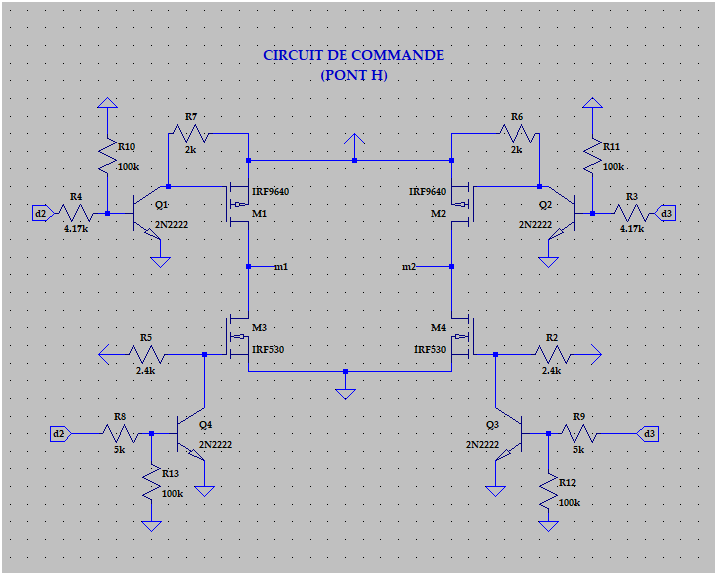
\includegraphics[width=1\linewidth]{images/pontH}
	\caption{Circuit de commande à deux étages des transistors}
	\label{fig:ponth}
\end{figure}

Le circuit de commande comporte quatre \acp{MOSFET}, quatre \acp{BJT} et douze résistances. Les deux \acp{MOSFET} côté haut sont à canal p à cause du pilotage simple des \acp{MOSFET} à canal p; les deux autres sont à canal n. Étant donné que pour ces transistors, $V_{GS}$ doit être supérieur à la tension de seuil en valeur absolue, nous tirons la tension d'alimentation à la grille du \textbf{pmos} et un étage supplémentaire à base d'un \textbf{npn} est ajouté. Quand le transistor bipolaire est passant, la tension au niveau du collecteur est environ $\SI{0.2}{\volt}$ rendant aussi le \textbf{pmos} passant.

Deux autres \textbf{npn} servent aussi à contrôler les \textbf{nmos} qui composent notre circuit. En effet, afin de totalement laisser passer le courant, il faut une tension de grille suffisante, bien supérieure aux $\SI{3.3}{\volt}$ fournies par le micro-contrôleur ; ce qui nous pousse à tirer cette tension d'une source extérieure(la source d'alimentation si possible). Quand le \ac{BJT} est passant, le \ac{MOSFET} est bloqué car la tension de grille qui est environ $\SI{0.2}{\volt}$ est loin derrière la tension de seuil. Quatre résistances de \SI{100}{\kilo\ohm} sont tirer à la masse au niveau des bases des \acp{BJT} afin d'éviter des connections flottantes. La valeur de ces résistances est choisie de façon à limiter le plus possible le courant de retour à la masse.

Pour la commande arduino, le moteur tourne dans un sens si la sortie $D2$ est \textbf{on} et la sortie $D3$ \textbf{off} ; il tourne dans le sens inverse si la sortie $D2$ est \textbf{off} et la sortie $D3$ \textbf{on}. Nous commençons par dimensionner les composants du circuit pour à la fin écrire le code de test du circuit avec arduino.

Bien que la tension nominale du moteur \ac{DC} soit de $\SI{9}{\volt}$, nous utiliserons la tension d'alimentation de $\SI{10}{\volt}$(nous sommes toujours dans la plage de fonctionnement). Notons que nous travaillons avec des contraintes, les transistors que nous utilisons sont surdimensionnés compte tenu de la difficulté de trouver des transistors répondant de près à nos exigences dans le marché. Il s'agit pour les \acp{BJT} du \textbf{2N2222A}, pour les \textbf{nmos} du \textbf{IRF540N} et pour les \textbf{pmos} du \textbf{IRF9540N} dont les spécifications techniques sont notées dans le classeur que nous avons cité dans le chapitre précédent. Pour la simulation, nous avons utilisé le \textbf{IRF9640} et le \textbf{IRF530} sur LTSpice ; le \textbf{IRF9530} et le \textbf{IRF540N} sur MultiSim. Ces différences sont dues à la disponibilité des modèles de ces composants sur ces logiciels! Toutefois, c'est possible de les installer pour plus de précision.

La fréquence par défaut des broches de l'Arduino nano 33 ble sense est de 500 Hz. Le courant maximal toléré par broche est de $\SI{10}{\milli\ampere}$ ; nous devons faire des calculs de façon à être très en dessous de cette valeur pour éviter d'endommager le micro-contrôleur.

Nous avons considéré un gain de saturation de $10$, nous avons imposé les valeurs des  résistances \textbf{R6 et R7} à $\SI{2000}{\ohm}$. Avec ces considération, nous avons les valeurs suivantes des résistances~:

\begin{table}[h]
	\centering
	\begin{tabular}{ll r l}
		\toprule
		Paire & Résistance & Valeur & Unité \\
		\midrule
		1 & R2, R5 & 2400,00 & $\Omega$ \\
		2 & R3, R4 & 4166,67 & $\Omega$ \\
		3 & R6, R7 & 2000,00 & $\Omega$ \\
		4 & R8, R9 & 5000,00 & $\Omega$ \\
		5 & R10, R11, R12, R13 & 100,00 & $k\Omega$ \\
		\bottomrule
	\end{tabular}
	\caption{Valeurs des résistances du circuit de commande}
\end{table}

Vu que la fréquence par défaut est faible, nous ignorons les effets capacitifs des \acp{MOSFET} dans les calculs de nos résistances. Ci-dessous, nous présentons le code de test du circuit de commande.

\section{Code test}
Ce code nous permet de vérifier que le pont en H fonctionne correctement avant sa fusion avec le modèle de reconnaissance vocale. Premièrement, l'on fait tourner le moteur dans un sens à la vitesse maximale souhaitée ; deuxièmement l'on change de sens de rotation en conservant l'ancienne vitesse et pour finir l'on baisse la vitesse de rotation avant de refaire la boucle.

\begin{lstlisting}[style=arduino]
	const int pin1 = 2;
	const int pin2 = 3;
	int PWM = 255; // vitesse maximale
	
	void setup() {
		Serial.begin(9600);
		pinMode(pin1, OUTPUT);
		pinMode(pin2, OUTPUT);
	}
	
	void loop() {
		if (PWM < 20){
			Serial.println("Vitesse maximale!!");
			PWM = 255;
		}
		
		analogWrite(pin1, PWM);
		analogWrite(pin2, 0);
		delay(5000);
		
		analogWrite(pin1, 0);
		analogWrite(pin2, PWM); // inversion de sens de rotation
		delay(5000);
		
		analogWrite(pin1, 0);
		analogWrite(pin2, 0);
		delay(5000);
		
		PWM = PWM - 65; // reduction de vitesse
		Serial.print("[Vitesse] : "); Serial.print(PWM); Serial.println("/255");
	}
	
\end{lstlisting}

\chapter{Présentation des résultats des tests du système}
\section{Test du circuit de commande}

\begin{figure}[H]
	\centering
	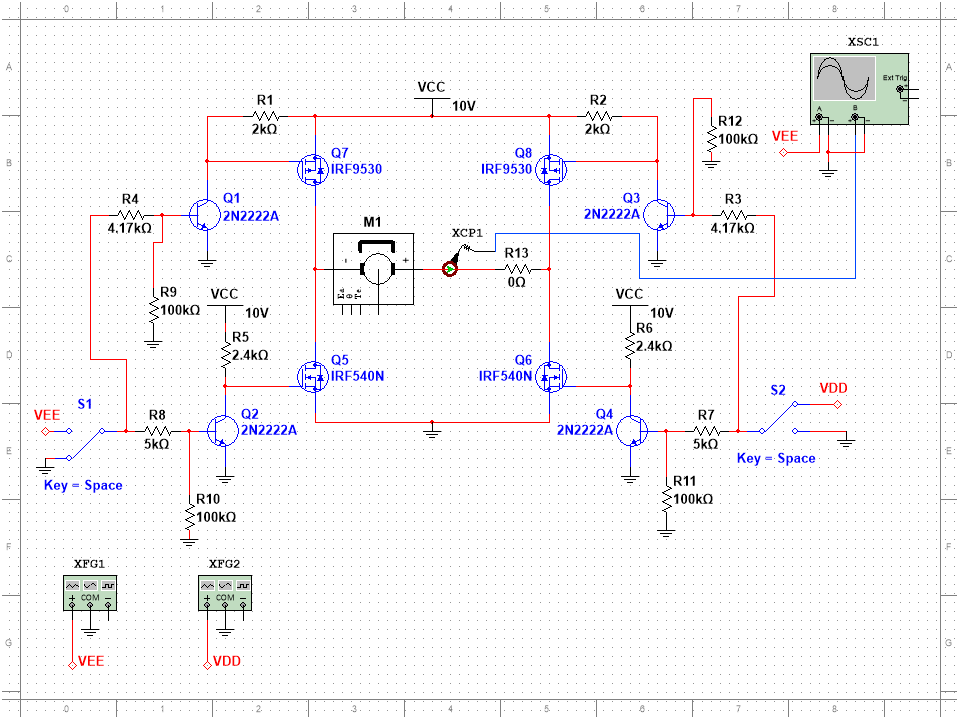
\includegraphics[width=1\textwidth]{./images/circuitMultisim}
	\caption{Circuit test sur MultiSim}
	\label{fig:circuitM}
\end{figure}

Deux types de tests ont été réalisés, une simulation interactive sur MultiSim dont la vidéo est disponible sur github dans le dossier \textbf{rapports}, et un essai pratique du circuit de commande. Afin de simuler le comportement de arduino sur MultiSim, nous avons utilisé deux générateurs de fonction carrées à rapport cyclique réglable de façon dynamique, pour une fréquence de $\SI{500}{\hertz}$. Le schéma ainsi que les réglages de cette simulation sont aussi disponible sur github dans le dossier \textbf{multisim\_simulation}. A partir de l'oscilloscope où le canal A (en rouge) représente la tension de commande et le canal B (en bleu) représente le courant d'armature du moteur(les réglages sont faites de telle sorte que $\SI{1}{\volt}$ corresponde à $\SI{1}{\milli\ampere}$ en utilisant l'instrument \textbf{Current clamp} de MultiSim) ; nous pouvons alors lire le courant d'induit maximal. Si nous commutons la commande grâce aux interrupteurs, nous remarquons que le sens du courant d'induit change aussi, ce qui veut dire que le sens de rotation a aussi changé.

\begin{figure}[H]
	\centering
	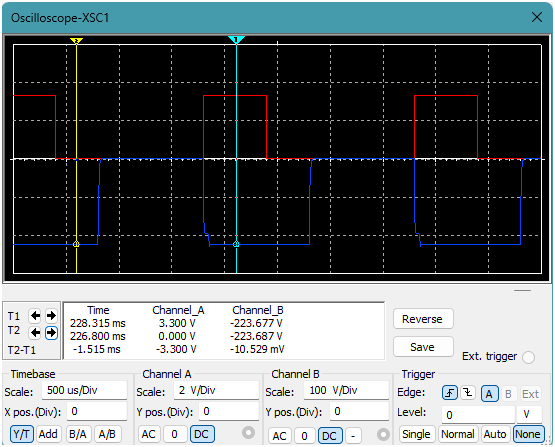
\includegraphics[width=0.7\linewidth]{images/oscillo1}
	\caption{Simulation MultiSim, premier sens de rotation}
	\label{fig:oscillo1}
\end{figure}

\begin{figure}[H]
	\centering
	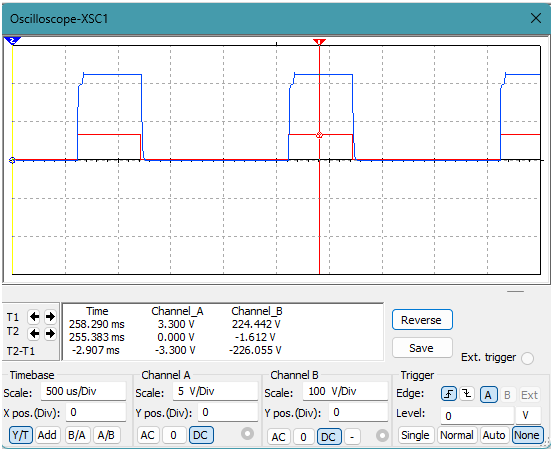
\includegraphics[width=0.7\linewidth]{images/oscillo2}
	\caption{Simulation MultiSim, inversion de sens de rotation($d=30\%$)}
	\label{fig:oscillo2}
\end{figure}

Quant au test au laboratoire, comme le montre l'essai d'une branche du pont en H que vous pouvez trouver sur Github, le système avait connu un problème dû au branchement des \textbf{pmos}. En effet, au lieu de connecter la source à \textbf{VCC}, nous connections plutôt le drain ; ainsi la diode interne du transistor conduisait directement peu importe la tension appliquée à la grille. D'où comme le \textbf{nmos} est passant d'après notre logique, c'est à dire $VDD=\SI{0}{\volt}$, et que le \textbf{pmos} est supposé être éteint($VEE=\SI{0}{\volt}$), le moteur tourne quand même, car nos connexions rendaient le \textbf{pmos} passant. Ce qui a eu pour conséquence de provoquer des courts-circuits quand tout le pont fonctionne, étant donné que deux interrupteurs non diagonaux se retrouvent fermés. Le schéma actuel n'a plus ce problème.

En progressant dans la simulation sur MultiSim pour une durée de \SI{6}{\second} environ et un rapport cyclique de $80\%$, nous constatons, en observant la durée pendant laquelle le signal de commande est nul, la présence d'un courant de sens opposé au courant d'induit. Quand le signal de commande est sur \textbf{OFF}, ce courant est de \SI{82.9}{\milli\ampere}, quand le signal de commande est sur \textbf{ON}, le courant d'induit est de \SI{163}{\milli\ampere}.

Ce courant dû à la nature inductive du moteur \ac{DC} peut être dangereux pour les transistors. Afin de le contenir, il est d'usage d'utiliser des diodes dites de \textbf{roue libre}. Dans notre cas, les transistors que nous utilisons implémentent déjà ces diodes de roue libre.

\begin{figure}[H]
	\centering
	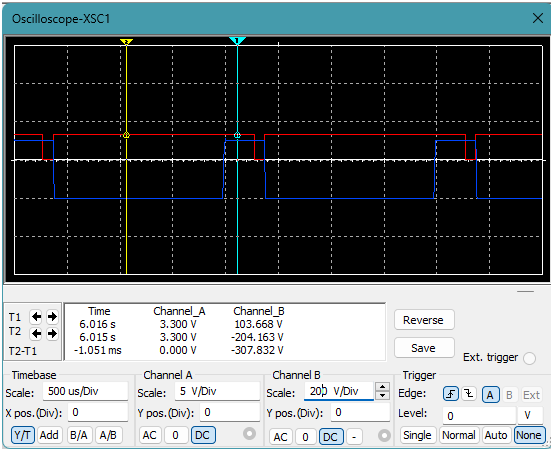
\includegraphics[width=0.7\textwidth]{images/reactionMoteur}
	\caption{Simulation MultiSim, réaction du moteur(d=$80\%$)}
	\label{fig:reactMoteur}
\end{figure}

\section{Test du modèle \ac{ML} sur arduino}
Après validation du circuit de commande, nous avons procédé au test du modèle embarqué sur arduino en conditions réelles. Le modèle reçoit en continu les données représentants les sons issus du microphone intégré ; puis classe la commande vocale prononcée comme membre d'une des six classes prévues(go, up, down, stop, left, inconnu) ; ensuite, une fois la commande validée, le microcontrôleur actionne les broches nécessaires qui contrôlent le moteur de façon à respecter la commande.

A l'aide du moniteur série, nous visualisons de façon interactive le fonctionnement du modèle dans le microcontrôleur à l'écran. Une vidéo de cette démonstration est disponible sur Github.

Dans l'ensemble, le système répond correctement(le volume auquel on s'exprime est important). Nous avons cependant observé quelques activations non désirées, où le modèle déclenche une action sans commande vocale explicite de l'opérateur, probablement dues aux bruits ambiants non pris en charge lors de l'entrainement.

Grâce au score de confiance seuil que nous avons fixé à 90\%, une prédiction n'est considérée par le microcontrôleur que si sa probabilité associée dépasse ce seuil, ce qui filtre la majorité des fausses activations.

\chapter{Conclusion}
\label{section:conclusion}
Au terme de ce travail, nous avons réussi à concevoir un système de contrôle vocal d'un moteur \ac{DC}, associant un modèle \textbf{TinyML} de classification multiclasse embarqué sur un  microcontrôleur Arduino Nano 33 \ac{BLE} Sense, et un circuit de commande en pont en H à base de transistors bipolaires et de \acp{MOSFET}. Ce projet nous a permis de mettre en pratique des notions relevant à la fois de l'électronique analogique, de l'apprentissage automatique et du traitement des signaux. Les tests réalisés sur la carte Arduino ont confirmé le bon fonctionnement du modèle, et la simulation interactive sur MultiSim approuve le circuit de commande que nous avons proposé. Les commandes vocales sont reconnues(avec quelques défauts), la commutation fonctionne aussi correctement, comme en témoignent nos vidéos postées sur la plateforme Github dans le dépôt publique \url{https://www.github.com/robohie/prog_python}.

Annoncé à l'introduction, l'usage du logiciel \textbf{KiCad} n'a pas malheureusement été évoqué dans ce rapport car nous n'avons pas su finir à temps la conception du \ac{PCB} pour notre circuit de commande. Vous trouverez quand même le projet sur Github, à l'intérieur du dossier dédié à l'emploi de ce logiciel.

Ce travail n'a cependant pas été exempt de difficultés. La conception du modèle deep learning a exigé de travailler avec des contraintes de mémoire et de calcul du microcontrôleur, rendant nécessaire un compromis entre la précision et la taille du modèle ; aussi faut-il souligner que tout a été fait sur mon ordinateur portable, prolongeant ainsi la durée d'entrainement. La meilleure pratique étant de le faire sur Google Colab. La difficulté à trouver sur le marché local des transistors répondant à nos exigences nous a obligés de surdimensionner les composants du circuit de commande. Enfin, lors des tests du modèle sur la carte arduino, nous avons observé quelques activations de commande spontanées, un défaut issu de l'entraînement du modèle, particulièrement le jeu de données d'entrainement.

Plusieurs perspectives se dégagent de ce travail. Le modèle d'apprentissage automatique pourrait être étendu à un vocabulaire plus large afin de couvrir de tâches complexes. Au lieu d'un simple moteur à courant continu à aimant permanent, le système pourrait piloter un moteur asynchrone, un relais, ou toute installation électromécanique.


%--------------------
%  ANNEXES
%--------------------
\appendix
\chapter{Modules Python utilisés}
Le jeu de données utilisé pour l'entraînement du modèle est le jeu de données Speech Commands~\cite{kaggle_speech_commands}. La bibliothèque utilisée pour l'inférence embarquée sur microcontrôleur est TensorFlow Lite for Microcontrollers~\cite{tflite_micro_github}.

Les modules suivants nous ont servi durant la conception du modèle et son entrainement : \textbf{Scikit-learn, Librosa, Numpy, Matplotlib, Tensorflow et Keras}.


%--------------------
%  BIBLIOGRAPHIE
%--------------------
\bibliographystyle{ieeetr}
\bibliography{rapport_ref}

\end{document}